% !TEX TS-program = XeLaTeX
\documentclass[a4paper,12pt,titlepage]{article}
\usepackage{fontspec} 						%字体配置包
\usepackage{enumerate}						%条目配置包
\usepackage{enumitem}
\usepackage{anysize}						%纸张边界留白配置包
\usepackage{indentfirst}					%设置首行缩进包
\usepackage{graphicx}						%图像插入包
\usepackage{float}							%图片强制定位
\usepackage{caption2}						%去掉插图名称中的冒号
\usepackage{fancyhdr}						%生成页眉
\usepackage{amsmath}
\usepackage{array}
\usepackage{amsthm}
\usepackage{mathrsfs}                % 英文花体字体
\usepackage{bm}                      % 数学公式中的黑斜体
\usepackage{bbding,manfnt}           % 一些图标,如 \dbend
\usepackage[colorlinks, linkcolor=black, anchorcolor=black, citecolor=black]{hyperref}
% \usepackage{lettrine}                % 首字下沉,命令\lettrine
% \def\attention{\lettrine[lines=2,lraise=0,nindent=0em]{\large\textdbend\hspace{1mm}}{}}
\usepackage{xeCJK}							%中英文混排
\usepackage[top=1in,bottom=1in,left=0.8in,right=0.8in]{geometry}
\pagestyle{fancy}

 % \marginsize{3.17cm}{3.17cm}{2.54cm}{2.54cm}	%边界留白设置


\setCJKmainfont{宋体} 							%宋体
\setCJKmonofont{楷体}
\setmainfont{Times New Roman} 					
% \XeTeXlinebreaklocale "zh"
% \XeTeXlinebreakskip = 0pt plus 1pt

\setlength{\parindent}{2em}					%缩进两个字
\linespread{1.5}
\setenumerate[1]{itemsep=1.5pt,partopsep=2pt,parsep=2pt,topsep=2pt}



\renewcommand{\today}{\number \year \ 年 \number \month \ 月 \number \day \ 日}
										%插入中文日期

% \renewcommand{\thefigure}{\arabic{section}.\arabic{figure}}

\renewcommand{\captionlabeldelim}{. }		%去掉插图名称中的冒号

\begin{document}
%%%%%%%%%% 定理类环境的定义 %%%%%%%%%%
%% 必须在导入中文环境之后
\newtheorem{example}{例}             % 整体编号
\newtheorem{algorithm}{算法}
\newtheorem{theorem}{定理}[section]  % 按 section 编号
\newtheorem{definition}{定义}
\newtheorem{axiom}{公理}
\newtheorem{property}{性质}
\newtheorem{proposition}{命题}
\newtheorem{lemma}{引理}
\newtheorem{corollary}{推论}
\newtheorem{remark}{注解}
\newtheorem{condition}{条件}
\newtheorem{conclusion}{结论}
\newtheorem{assumption}{假设}

%%%%%%%%%% 一些重定义 %%%%%%%%%%
\renewcommand{\contentsname}{目录}     % 将Contents改为目录
\renewcommand{\abstractname}{摘要}     % 将Abstract改为摘要
\renewcommand{\refname}{参考文献}      % 将References改为参考文献
\renewcommand{\indexname}{索引}
\renewcommand{\figurename}{图}
\renewcommand{\tablename}{表}
\renewcommand{\appendixname}{附录}
\renewcommand{\proofname}{证明}
\renewcommand{\algorithm}{算法}




% \setkeys{Gin}{width=0.8\textwidth}				%设置图片大小

\title{\huge{双杆复合摆的计算机模拟}}
\author{ 谌阳平 \\
清华大学 \quad 工程物理系 \quad 核91 \quad 2009011737}
\date{\today}
\maketitle

\tableofcontents



\begin{abstract}
以拉格朗日力学为基础,通过计算双杆复合摆系统的拉格朗日量,求解拉格朗日方程,求得双杆复合摆系统的运动微分方程,分别采用预估-校正的Verlet算法、经典四阶Runge-Kutta算法和自适应时间步长的四阶Runge-Kutta算法,通过计算机模拟的方法仿真双杆复合摆的运动。并通过引入空气阻尼,研究有阻尼情况下的双杆复合摆系统的运动特性。

\vskip 0.1in
\begin{flushleft}
\begin{minipage}{5.7in}
\noindent{{\textbf{【关键词】}} 双杆复合摆;拉格朗日方程;空气阻尼。}\\
\end{minipage}
\end{flushleft}
\end{abstract}


\section{双杆复合摆问题描述} % (fold)
\label{sec:Discription_}
双杆复合摆系统构成如图~\ref{fig:system}所示。
\begin{figure}[htpb]
\centering
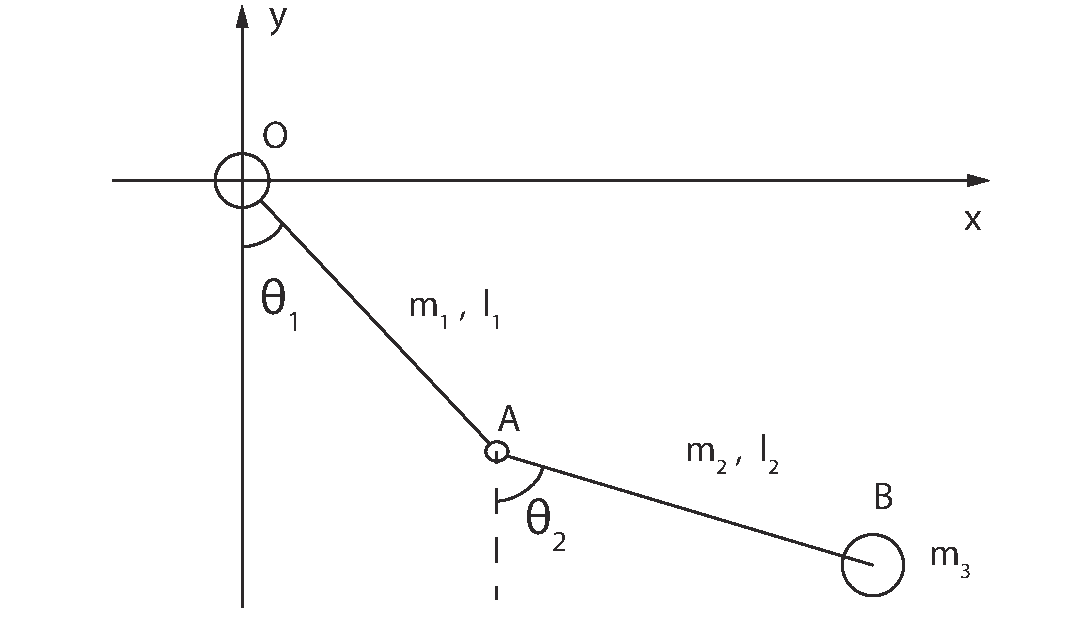
\includegraphics[width=\textwidth]{./system.pdf}
\caption[Caption for LOF]{双杆复合摆系统示意图}
\label{fig:system}
\end{figure}
双杆系统的杆的重量不可忽略,所以整个系统由质量为$m_1$和$m_2$,长度为$l_1$和$l_2$的两根刚性杆和质量为$m_3$的体积可忽略的小球组成,两杆之间用理想无摩擦的铰连接。一般情况下,运动角度$\theta_1$和$\theta_2$的范围并不局限于小角度,且由于双杆均有质量,因此系统不是简单的简谐振动系统。


% section Discription_ (end)

\section{拉格朗日力学简介} % (fold)
\label{sec:Lagrange Mechanics}
拉格朗日力学是以拉格朗日方程为第一性原理,从整体考察体系的运动规律,挑出真实运动,具有直观紧凑的形式$\delta S=0$,且Hamilton原理着眼于能量,除了求解容易外,还利于推广。

由牛顿力学方程组和虚功原理,可以退出达朗贝尔-拉格朗日方程
\begin{equation}
\label{eq:dle}
	\sum_{i=1}^n \left(\vec{F}_i-m_i\ddot{\vec{r}}_i\right)\cdot \delta\vec{r}_i=0
\end{equation}
它的物理意义是:所有质点所受的主动力和惯性力的虚功的代数和为0,其中$\delta$为等时变分,$F_i$质点$i$所受主动力。该方程也可推广到连续质量分布体系,只需将求和变为相应积分即可。

设体系的广义坐标为$q_\alpha~(\alpha=0,1,...,s)$,$s$为系统自由度,从达朗贝尔-拉格朗日方程出发,推导拉格朗日方程。
显然,达朗贝尔-拉格朗日方程与下方程等价
\begin{equation}
\label{eq:dle2}
	\sum_{\alpha=1}^s\left[\sum_{i=1}^n \vec{F}_i\cdot\frac{\partial \vec{r}_i}{\partial q_{\alpha}}-\sum_{i=1}^n m_i\ddot{\vec{r}}_i\cdot\frac{\partial \vec{r}_i}{\partial q_\alpha} \right]\cdot \delta q_\alpha=0
\end{equation}
处理与质点加速度相关的第二项
\begin{align}
	\sum_{i=1}^n m_i \ddot{\vec{r}}_i\cdot\frac{\partial \vec{r}_i}{\partial q_\alpha} &= \sum_{i=1}^n m_i\left[ \frac{\mathrm{d}}{\mathrm{d}t}\left(\dot{\vec{r}}_i\cdot\frac{\partial \vec{r}_i}{\partial q_\alpha} \right)-\dot{\vec{r}}_i\cdot\frac{\mathrm{d}}{\mathrm{d}t}\frac{\partial \vec{r}_i}{\partial q_\alpha} \right]\notag\\
	&=\sum_{i=1}^n m_i\left[ \frac{\mathrm{d}}{\mathrm{d}t}\left(\dot{\vec{r}}_i\cdot\frac{\partial \vec{r}_i}{\partial \dot{q}_\alpha} \right)-\dot{\vec{r}}_i\cdot\frac{\partial \dot{\vec{r}}_i}{\partial q_\alpha} \right]\notag\\
	&=\frac{\mathrm{d}}{\mathrm{d}t}\frac{\partial T}{\partial \dot{q}_\alpha}-\frac{\partial T}{\partial q_\alpha}
	\label{eq:mr}
\end{align}
其中$T=\frac{1}{2}\sum_{i=1}^n m_i\dot{\vec{r}}_i^2$为动能,以上运算利用了两个经典拉格朗日关系
\begin{equation}
	\frac{\partial \dot{\vec{r}}_i}{\partial \dot{q}_\alpha}=\frac{\partial \vec{r}_i}{\partial q_\alpha} \quad
	\frac{\mathrm{d}}{\mathrm{d}t}\frac{\partial \vec{r}_i}{\partial q_\alpha}=\frac{\partial \dot{\vec{r}}_i}{\partial q_\alpha} \notag
\end{equation}
所以,方程(\ref{eq:dle2})就化为
\begin{equation}
\label{eq:ele}
	\sum_{\alpha=1}^s\left( Q_\alpha+\frac{\partial T}{\partial {q}_\alpha}-\frac{\mathrm{d}}{\mathrm{d}t}\frac{\partial T}{\partial \dot{q}_\alpha} \right)=0
\end{equation}
其中$Q_\alpha=\sum_{i=1}^n \vec{F}_i\cdot\frac{\partial \vec{r}_i}{\partial q_{\alpha}}$称为主动力对应于广义坐标$q_\alpha$的广义力。在约束完整的条件下,由于$\delta q_\alpha$是相互独立的,由方程(\ref{eq:ele})就得到基本形式的拉格朗日方程
\begin{equation}
\label{eq:leb}
	\frac{\mathrm{d}}{\mathrm{d}t}\frac{\partial T}{\partial \dot{q}_\alpha}-\frac{\partial T}{\partial q_\alpha}=Q_\alpha\quad \alpha=1,2,...,s
\end{equation}
方程(\ref{eq:leb})对于理想、完整的力学体系普遍成立。

在主动力为有势力的情况下$\vec{F}_i=-\frac{\partial V(q,t)}{\partial \vec{r}_i} $,$V$为使能,广义力可表为
\begin{equation}
	Q_\alpha=\sum_{i=1}^n \vec{F}_i\cdot \frac{\partial \vec{r}_i}{\partial q_\alpha}=\sum_{i=1}^{n}\left(-\frac{\partial V(q,t)}{\partial \vec{r}_i}\right)\cdot\frac{\partial \vec{r}_i}{\partial q_\alpha}=-\frac{\partial V}{\partial q_\alpha}
\end{equation}
于是方程(\ref{eq:leb})化为
\begin{equation}
\label{eq:le1}
	\frac{\mathrm{d}}{\mathrm{d}t}\frac{\partial L}{\partial \dot{q}_\alpha}-\frac{\partial L}{\partial q_\alpha}=0 \quad \alpha=1,2,...,s
\end{equation}
即第二类拉格朗日方程。其中$L=T-V$称为拉格朗日函数。

若考虑存在非保守力$\vec{f}_i$的情况,则将非保守力看做主动力的一部分。则广义力为
\begin{equation}
	Q_\alpha=\sum_{i=1}^n \left(\vec{F}_i+\vec{f}_i\right)\cdot \frac{\partial \vec{r}_i}{\partial q_\alpha}=-\frac{\partial V}{\partial q_\alpha}+Q'_\alpha
\end{equation}
其中
\begin{equation}
\label{eq:force}
	Q'_\alpha=\sum_{i=1}^n \vec{f}_i\cdot \frac{\partial \vec{r}_i}{\partial q_\alpha}
\end{equation}为非保守力对应的广义力,方程(\ref{eq:leb})化为
\begin{equation}
\label{eq:le2}
	\frac{\mathrm{d}}{\mathrm{d}t}\frac{\partial L}{\partial \dot{q}_\alpha}-\frac{\partial L}{\partial q_\alpha}=Q'_\alpha \quad \alpha=1,2,...,s
\end{equation}
即存在非有势力体系的拉格朗日方程。
% section Lagrange Mechanics (end)

\section{双杆复合摆系统的力学分析} % (fold)
\label{sec:anlysis of mechanics}
\subsection{无空气阻力的双杆复合摆系统}
如图~\ref{fig:system}所示。显然,系统自由度$s=2$,且$\theta_1$和$\theta_2$相互独立。所以选取$\theta_1$和$\theta_2$作为独立广义坐标。

首先计算双杆复合摆体系的动能$T(\vec{q},\dot{\vec{q}},t) $和势能$V(\vec{q},t) $。
杆1的运动为围绕O点的圆周运动,因此需要计算杆的转动能量。杆1对以O点为中心的转动惯量
\begin{equation*}
	J_1=\frac{1}{3}m_1l_1^2
\end{equation*}
所以根据转动能量的计算公式
\begin{equation}
	T_{1}=\frac{1}{2}J_1\dot{\theta}_1^2=\frac{1}{6}m_1l_1^2\dot{\theta}_1^2
\end{equation}
对于杆2,由于其运动是转动和平动的复合运动,因此其动能是其质心平动动能和以质心为中心的转动动能的和。杆2以质心为中心的转动惯量为
\begin{equation*}
	J_2=\frac{1}{12}m_2l_2^2
\end{equation*}
质心坐标为
\begin{equation*}
	x_2=l_1\sin{\theta_1}+\frac{l_2}{2}\sin{\theta_2} \quad
	y_2=-l_1\cos{\theta_1}-\frac{l_2}{2}\cos{\theta_2} 
\end{equation*}
所以
\begin{align}
	T_{2}&=\frac{1}{2}J_2\dot{\theta}_2^2+\frac{1}{2}m_2\left(\dot{x}_2^2+\dot{y}_2^2\right) \notag\\
	&=\frac{1}{6}m_2\left(3l_1^2\dot{\theta}_1^2+3l_1l_2\dot{\theta}_1\dot{\theta}_2\cos{(\theta_2-\theta_1)}+l_2^2\dot{\theta}_2^2\right)
\end{align}
对于B端的摆锤,其坐标为
\begin{equation*}
	x_3=l_1\sin{\theta_1}+l_2\sin{\theta_2} \quad
	y_3=-l_1\cos{\theta_1}-l_2\cos{\theta_2} \notag
\end{equation*}
所以,摆锤的动能为
\begin{align}
	T_{3}&=\frac{1}{2}m_3\left(\dot{x}_3^2+\dot{y}_3^2 \right)\notag\\
	&=\frac{1}{2}m_3\left(l_1^2\dot{\theta}_1^2+2l_1l_2\dot{\theta}_1\dot{\theta}_2\cos{(\theta_2-\theta_1)}+l_2^2\dot{\theta}_2^2 \right)
\end{align}
所以双杆复合摆系统的动能为
\begin{align}
	T&=T_1+T_2+T_3 \notag\\
	&=\frac{1}{6}\left(l_1^2\left(m_1+3\left(m_2+m_3 \right) \right)\dot{\theta}_1^2+3\left(m_2+2m_3 \right)l_1l_2\dot{\theta}_1\dot{\theta}_2\cos{(\theta_2-\theta_1)}+\left(m_2+3m_3\right)l_2^2\dot{\theta}_2^2 \right)
\end{align}
复合摆系统的势能为重力势能,其表达式为
\begin{equation}
	V=-\frac{1}{2} g \left(l_2 \left(m_2+2 m_3\right) \cos{\theta_2}+l_1
   \left(m_1+2 \left(m_2+m_3\right)\right) \cos{\theta_1}\right)
\end{equation}
所以系统的拉格朗日函数为
\begin{align}
\label{eq:lv}
	L=&T-V \notag\\
	=&\frac{1}{6} ( 3 g ((m_2+2 m_3) l_2 \cos{\theta_2}+ (m_1+2 (m_2+m_3))l_1 \cos{\theta_1})+(m_1+3(m_2+m_3)) l_1^2 \dot{\theta}_1^2 \notag \\
    &+ (m_2+3 m_3) l_2^2\dot{\theta}_2^2+3(m_2+2m_3) l_1 l_2 \dot{\theta}_1 \dot{\theta}_2 \cos{(\theta_2-\theta_1)} )
\end{align}
将公式(\ref{eq:lv})代入拉格朗日方程(\ref{eq:le1}),化简可得以$\ddot{\theta}_1 $和$\ddot{\theta}_2 $为变量的方程组。化为矩阵形式为
\begin{equation}
\label{eq:me}
	A_{2\times 2}\vec{x}=\vec{b}
\end{equation}
其中
\begin{align}
	\label{eq:parx}
	&\vec{x}=\left(\ddot{\theta}_1,\ddot{\theta}_2\right)\\
	\label{eq:parA}
	&\begin{cases}
		A_{11}=\frac{1}{3}(m_1+3(m_2 + m_3))l_1^2 \\
		A_{12}=\frac{1}{2}(m_2+2m_3)l_1l_2\cos{(\theta_2-\theta_1)} \\
		A_{21}=\frac{1}{2}(m_2+2m_3)l_1l_2\cos{(\theta_2-\theta_1)} \\
		A_{22}=\frac{1}{3}(m_2+3 m_3)l_2^2 
	\end{cases}\\
	\label{eq:parb}
	&\begin{cases}
		b_1=-\left(\frac{m_1}{2}+m_2+m_3\right)l_1g\sin{\theta_1}+\left(\frac{m_2}{2}+m_3\right)l_1l_2\dot{\theta}_2^2\sin{(\theta_2-\theta_1)}\\
		b_2=-l_2 \left(\frac{m_2}{2}+ m_3\right) \left(g \sin{\theta_2}+l_1\dot{\theta}_1^2 \sin \left(\theta_2-\theta_1\right)\right)
	\end{cases}
\end{align}
根据克莱姆法则,方程的解为
\begin{equation}
\label{eq:re}
	\begin{cases}
		\ddot{\theta}_1&=\frac{b_1A_{22}-b_2A_{12}}{A_{11}A_{22}-A_{12}A_{21}}\\
		\ddot{\theta}_2&=\frac{b_2A_{11}-b_1A_{21}}{A_{11}A_{22}-A_{12}A_{21}}
	\end{cases}
\end{equation}
由于在模拟过程中,每一时刻的$\theta_1$、$\theta_2$、$\dot{\theta}_1$、$\dot{\theta}_2$已知,因此可以根据公式(\ref{eq:re})求得角加速度,从而进行模拟。

\subsection{有空气阻力的双杆复合摆系统}
实际的双杆复合摆系统由于不可能在真空中运行,因此最有常见的非保守力是空气阻力。空气阻力的大小与运动物体的几何形状、截面积、相对运动速度均有关系,且函数关系不能用简单的函数表示。为简化计算,本次模拟认为空气阻力只与相对运动速度和截面积相关,且认为双杆复合摆中杆的截面积相同,忽略摆锤的空气阻力。所以,空气阻力在杆上单位长度的力密度为
\begin{equation}
\label{eq:af}
	\vec{f}=-\mu \frac{(\vec{v}\cdot\hat{\theta})^3}{|\vec{v}\cdot\hat{\theta}|}
\end{equation}
其中,$v$为阻力作用处的杆微元的速度,$\hat{\theta}$为杆的法向单位向量,所以可知$\vec{f}$大小与杆速度的法向分量的平方成正比,方向与杆法相速度相反。

根据有主动力的拉格朗日方程(\ref{eq:le2}),我们需要根据公式(\ref{eq:force})计算空气阻力在广义坐标下的广义力$Q'_\alpha$。

首先将公式(\ref{eq:force})推广到一维连续体系,得
\begin{equation}
\label{eq:force1}
	Q'_\alpha=\int_0^l \vec{f}(\vec{r})\cdot\frac{\partial \vec{r}}{\partial q_\alpha}\mathrm{d}x\quad \alpha=1,2,...,s
\end{equation}
其中$\vec{f}$为主动力的力密度。

作用在杆1上的空气阻力可以表示为
\begin{equation}
\label{eq:af11}
	\vec{f}_1(x)=-\mu x^2 \frac{\dot{\theta}_1^3}{|\dot{\theta}_1|}\hat{\theta}_1\quad x\in [0,l_1]
\end{equation}
要计算作用在杆2的空气阻力,首先需要计算杆2上单元的速度表达式
\begin{align}
	\vec{v}_2(x)&=\dot{x}\hat{e}_x+\dot{y}\hat{e}_y \notag \\
	&=\left(l_1\dot{\theta}_1\cos{\theta_1}+x\dot{\theta_2}\cos{\theta_2} \right)\hat{e}_x+\left(l_1\dot{\theta}_1\sin{\theta_1}+x\dot{\theta_2}\sin{\theta_2} \right)\hat{e}_y
\end{align}
根据矢量运算法则和各个单位矢量的角度关系
\begin{equation}
	\hat{e}_x\cdot\hat{\theta}_1=\cos{\theta}_1 \quad
	\hat{e}_y\cdot\hat{\theta}_1=\sin{\theta}_1	\quad
	\hat{e}_x\cdot\hat{\theta}_2=\cos{\theta}_2 \quad
	\hat{e}_y\cdot\hat{\theta}_2=\sin{\theta}_2
\end{equation}
所以
\begin{align}
\label{eq:vv}
	\vec{v}_2(x)\cdot\hat{\theta}_2&=\dot{x}\hat{e}_x+\dot{y}\hat{e}_y \notag \\
	&=\left(l_1\dot{\theta}_1\cos{\theta_1}+x\dot{\theta_2}\cos{\theta_2} \right)\cos{\theta}_2+\left(l_1\dot{\theta}_1\sin{\theta_1}+x\dot{\theta_2}\sin{\theta_2} \right)\sin{\theta}_2 \notag \\
	&=x\dot{\theta}_2+l_1\dot{\theta}_1\cos{(\theta_2-\theta_1)}
\end{align}
将方程(\ref{eq:vv})代入公式(\ref{eq:af}),得
\begin{equation}
\label{eq:af21}
	\vec{f}_2(x)=-\mu\frac{(x\dot{\theta}_2+l_1\dot{\theta}_1\cos{(\theta_2-\theta_1)})^3}{|x\dot{\theta}_2+l_1\dot{\theta}_1\cos{(\theta_2-\theta_1)}|}\hat{\theta}_2
\end{equation}
另外,显然有
\begin{align}
\label{eq:af12}
	\frac{\partial \vec{r}}{\partial \theta_1}=&\begin{cases}
		x\cos{\theta_1}\hat{e}_x+x\sin{\theta_1}\hat{e}_y & \text{杆1},x\in[0,l_1] \\
		l_1\cos{\theta_1}\hat{e}_x+l_1\sin{\theta_1}\hat{e}_y & \text{杆2},x\in[0,l_2]
	\end{cases}\\
\label{eq:af22}
	\frac{\partial \vec{r}}{\partial \theta_2}=&\begin{cases}
		0 & \text{杆1},x\in[0,l_1] \\
		x\cos{\theta_2}\hat{e}_x+x\sin{\theta_2}\hat{e}_y & \text{杆2},x\in[0,l_2]
	\end{cases}
\end{align}
将方程(\ref{eq:af11})~(\ref{eq:af12})~(\ref{eq:af21})~(\ref{eq:af22})代入方程(\ref{eq:force1}),可得空气阻力对应的广义力$Q'_1$和$Q'_2$。代入存在非有势力的拉格朗日方程(\ref{eq:le2}),化简同样可得以$\ddot{\theta}_1$和$\ddot{\theta}_2$为变量的方程组。矩阵形式同样可表为方程(\ref{eq:me}),系数矩阵$A$和变量向量$\vec{x}$与公式(\ref{eq:parA})~(\ref{eq:parx})相同,常数向量$\vec{b}'$为
\begin{equation}
	\begin{cases}
		b'_1=b_1+Q'_1\\
		b'_2=b_2+Q'_2
	\end{cases}
\end{equation}
其中$b_1$和$b_2$由公式(\ref{eq:parb})给出。

\subsection{两种情况下双杆复合摆的关系}
可以看出,无空气阻力的复合摆是有空气阻力情况的一种特例,在实际模拟计算过程中,可以利用有空气阻力的复合摆模拟程序,通过令空气阻力系数$\mu=0$的方法,获得无空气阻力的复合摆运动。只是由于以上计算中所有参量的均采用双精度浮点数,因此$\mu=0$的情况依然会引入一个小的不确定的空气阻力。如果采取合适的算法,该误差不会累积,因此不会对模拟结果造成严重影响。
% section:anlysis of mechanics (end)

\section{双杆复合摆模拟程序算法简介} % (fold)

\subsection{Verlet算法}
由于双杆复合摆系统在相空间并不一定是闭合的曲线,因此采用Euler法和Euler-Cromer方法均可能导致模拟误差累积导致模拟结果错误。因此采用收敛性更好的Verlet算法,即
\begin{equation}
\label{eq:verlet}
	\begin{cases}
		\theta_{\alpha,n+1}=\theta_{\alpha,n}+\dot{\theta}_{\alpha,n}\Delta t+\frac{1}{2}\ddot{\theta}_{\alpha,n}(\Delta t)^2\\
		\dot{\theta}_{\alpha,n+1}=\dot{\theta}_{\alpha,n}+\frac{1}{2}(\ddot{\theta}_{\alpha,n+1}+\ddot{\theta}_{\alpha,n})\Delta t
	\end{cases}
	\quad \alpha = 1,2
\end{equation}
从方程组(\ref{eq:verlet})可以看出,每次计算需要先计算出$\ddot{\theta}_{\alpha,n+1}$,然而由于$\ddot{\theta}_{\alpha,n+1}$的表达式很复杂,难以反解出其关于已知量的表达式。因此采用预估-校正法,即首先采用Euler法计算角速度
\begin{equation}
	\begin{cases}
		\theta_{\alpha,n+1}=\theta_{\alpha,n}+\dot{\theta}_{\alpha,n}\Delta t+\frac{1}{2}\ddot{\theta}_{\alpha,n}(\Delta t)^2\\
		\dot{\bar{\theta}}_{\alpha,n+1}=\dot{\theta}_{\alpha,n}+\ddot{\theta}_{\alpha,n}\Delta t
	\end{cases}
	\quad \alpha = 1,2
\end{equation}
然后利用估计的角速度$\dot{\bar{\theta}}_{\alpha,n+1}$和更新后的$\theta_{\alpha,n+1}$重新计算$\ddot{\bar{\theta}}_{\alpha,n+1}$,最后代入方程组(\ref{eq:verlet}),得到预估-校正的Verlet算法
\begin{equation}
\label{eq:verlet2}
	\begin{cases}
		\theta_{\alpha,n+1}=\theta_{\alpha,n}+\dot{\theta}_{\alpha,n}\Delta t+\frac{1}{2}\ddot{\theta}_{\alpha,n}(\Delta t)^2\\
		\dot{\theta}_{\alpha,n+1}=\dot{\theta}_{\alpha,n}+\frac{1}{2}(\ddot{\bar{\theta}}_{\alpha,n+1}+\ddot{\theta}_{\alpha,n})\Delta t
	\end{cases}
	\quad \alpha = 1,2
\end{equation}

Verlet算法流程图如图~\ref{fig:process_Verlet}所示。
\begin{figure}[H]
\centering
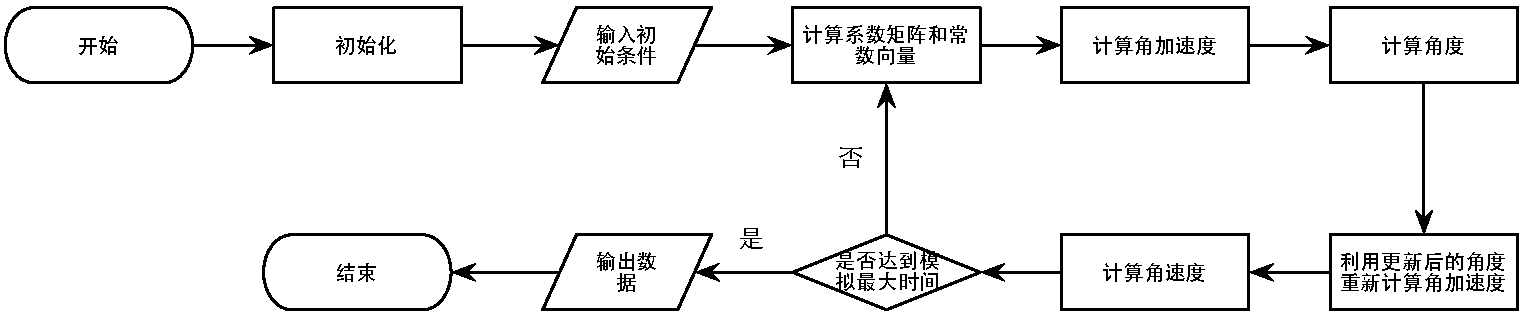
\includegraphics[height=0.13\textheight]{./process.pdf}
\caption[Caption for LOF]{Verlet算法流程图}
\label{fig:process_Verlet}
\end{figure}


\subsection{经典四阶Runge-Kutta方法}
Verlet方法实际上是改进后的Euler方法,其计算思想是利用Taylor展开,计算高阶偏导数,从而构造高阶的计算方法。从Taylor展开的表达式来看,计算一步时需要计算很多偏导数。特别是当函数结构及相应偏导数比较复杂时,这类高阶方法是不实用的。从本文涉及的双杆复合摆问题来看,利用拉格朗日方法计算得到的角加速度(即广义坐标的二阶导数)已经很复杂,三阶导数更加难以表达,因此很难通过Taylor展开的方法构造更高阶的方法。采用上述构造高阶方法的思想,但又不计算偏导数,由此导出了Runge-Kutta方法。
Runge-Kutta方法可以构造高阶精度的方法来求解初值问题,因此一直受到人们的重视。至今仍未实际应用的重要方法。

$m$元一阶常微分方程组的经典四阶Runge-Kutta方法的具体计算格式如下
\begin{equation}
\label{eq:RK}
	\begin{cases}
		y_{i,n+1}=y_{i,n}+\frac{1}{6}h(k_{i,1}+2k_{i,2}+2k_{i,3}+k_{i,4}) \\
		k_{i,1}=f_i(\vec{x}_n,\vec{y}_n)\\
		k_{i,2}=f_i(\vec{x}_n+\frac{1}{2}h,\vec{y}_n+\frac{1}{2}h\vec{k}_1)\\
		k_{i,2}=f_i(\vec{x}_n+\frac{1}{2}h,\vec{y}_n+\frac{1}{2}h\vec{k}_2)\\
		k_{i,2}=f_i(\vec{x}_n+h,\vec{y}_n+h\vec{k}_3)\\
	\end{cases}
	\quad i = 1,2,...,m
\end{equation}
其中,$\vec{x}_n=(x_{1,n},x_{2,n},...,x_{m,n})^T~,\vec{y}_n=(y_{1,n},y_{2,n},...,y_{m,n})^T~,\vec{k_i}=(k_{i,1},k_{i,2},...,k_{i,m})^T$。

对于高阶常微分方程组,如本文所涉及的双杆复合摆系统满足的方程组
\begin{equation}
\label{eq:fg1}
	\begin{cases}
		\ddot{\theta}_1=f_1(\theta_1,\theta_1,\dot{\theta}_1,\dot{\theta}_2)\\
		\ddot{\theta}_2=f_2(\theta_1,\theta_1,\dot{\theta}_1,\dot{\theta}_2)\\
	\end{cases}
\end{equation}
需要进行如下构造。

\noindent 取
\begin{equation}
	 	y_1=\dot{\theta}_1~,
	 	y_2=\dot{\theta}_2~,
	 	y_3=\theta_1~,
	 	y_4=\theta_2
\end{equation}
则方程组(\ref{eq:fg1})化为
\begin{equation}
	\begin{cases}
		\dot{y}_1=f_1(y_1,y_2,y_3,y_4)\\
		\dot{y}_2=f_2(y_1,y_2,y_3,y_4)\\
		\dot{y}_3=y_1\\
		\dot{y}_4=y_2\\
	\end{cases}
\end{equation}
按照方程组(\ref{eq:RK})所给方法,即为双杆复合摆问题的经典四阶Runge-Kutta方法。程序流程图如图~\ref{fig:process_RK}所示。

\begin{figure}[H]
\centering
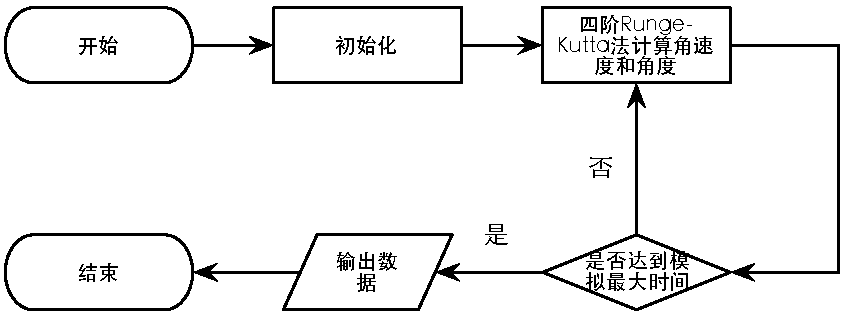
\includegraphics[height=0.13\textheight]{./process_RK.pdf}
\caption[Caption for LOF]{经典四阶Runge-Kutta算法流程图}
\label{fig:process_RK}
\end{figure}


\subsection{自适应时间步长算法(Adaptive Stepsize Method)}
双杆复合摆系统是准周期的震荡系统,存在动能和势能的转换。由于系统的常微分方程是关于时间的,因此时间步长的选取极大地影响到最终计算结果。

然而实际上,由于不同的角度和角速度条件下,计算的误差有数个量级的差别。因此对于某一给定的计算精度,不同时间所需的时间步长是不同的。在定步长条件下,长步长选取会导致误差变大,短步长会导致计算时间过长。因此,通过对当前条件计算不同的时间步长是兼顾计算速度和计算精度的方法之一。

四阶Runge-Kutta法为四阶收敛,因此其截断误差为
\begin{equation}
	T_{n+1}=O(h^{5}) \notag
\end{equation}
若使用五阶Runge-Kutta算法,则截断误差为
\begin{equation}
	\bar{T}_{n+1}=O(h^{6}) \notag
\end{equation}
因此,
\begin{equation}
	T_{n+1}(h)\approx|y_{n+1}-\bar{y}_{n+1}|\approx Kh^5 \notag
\end{equation}
若采用新的步长$qh$,则
\begin{equation}
	T_{n+1}(qh)\approx Kq^5h^5 \approx q^5|y_{n+1}-\bar{y}_{n+1}| \notag
\end{equation}
因此,选择期望截断误差为$\Delta_0$,设$\Delta=y_{n+1}-\bar{y}_{n+1}$,所以
\begin{equation}
	T_{n+1}(qh)\approx q^5|\Delta| < \Delta_0 \notag
\end{equation}
所以,
\begin{equation}
	q<\left( \frac{\Delta_0}{\Delta} \right)^{\frac{1}{5}} \notag
\end{equation}
则调整后的步长为
\begin{equation}
	h'=qh<h\left|\frac{\Delta_0}{\Delta}\right|^{\frac{1}{5}} \notag
\end{equation}

进行误差控制的通用技巧是Runge-Kutta-Fehlberg方法。这个技巧是采用5阶Runge-Kutta方法
\begin{equation}
	\bar{y}_{n+1}=y_n+h\left( \frac{16}{135}K_1+\frac{6656}{12825}K_3+\frac{28561}{56430}K_4-\frac{9}{50}K_5+\frac{2}{55}K_6 \right) \notag
\end{equation}
来估计四阶Runge-Kutta方法
\begin{equation}
	y_{n+1}=y_n+h\left( \frac{25}{216}K_1+\frac{1408}{2565}K_3+\frac{2197}{4104}K_4-\frac{1}{5}K_5 \right) \notag
\end{equation}
的局部截断误差,其中
\begin{equation}
	\begin{cases}
		K_1=f(x_n,y_n) \\
		K_2=f(x_n+\frac{h}{4},y_n+\frac{h}{4}K_1) \\
		K_3=f(x_n+\frac{3h}{8},y_n+\frac{3}{32}hK_1+\frac{9}{32}hK_2) \\
		K_4=f(x_n+\frac{12}{13}h,y_n+\frac{1932}{2197}hK_1-\frac{7200}{2197}hK_2+\frac{7296}{2197}hK_3) \\
		K_5=f(x_n+h,y_n+\frac{439}{216}hK_1-8hK_2+\frac{3680}{513}hK_3-\frac{845}{4104}hK_4) \\
		K_6=f(x_n+\frac{h}{2},y_n-\frac{8}{27}hK_1+2hK_2-\frac{3544}{2565}hK_3+\frac{1859}{4104}hK_4-\frac{11}{40}hK_5) 
	\end{cases}
	\notag
\end{equation}
注意到,4阶方法中$K_i$完全出现在5阶方法中。此种方法成为嵌入方法。

通常选取q为
\begin{equation}
	q=\left|\frac{\Delta_0}{2\Delta}\right|^{\frac{1}{5}}=0.87\left|\frac{\Delta_0}{\Delta}\right|^{\frac{1}{5}}
\end{equation}

采用自适应时间步长算法(Adaptive Stepsize Method)的程序流程图如图~\ref{fig:process_ASM}所示。
\begin{figure}[H]
\centering
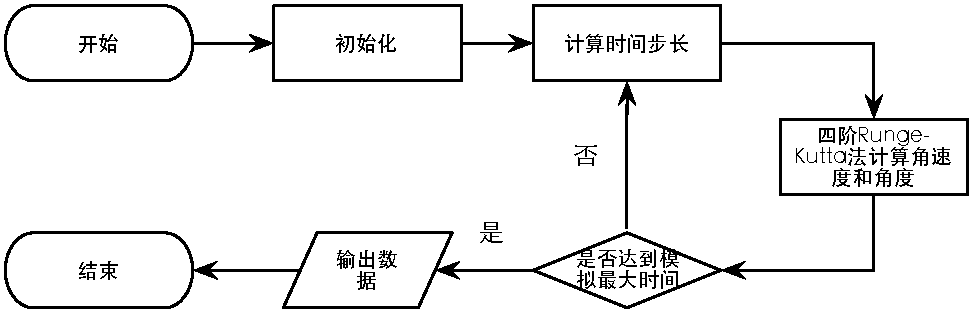
\includegraphics[height=0.13\textheight]{./process_ASM.pdf}
\caption[Caption for LOF]{自适应时间步长算法流程图}
\label{fig:process_ASM}
\end{figure}

\subsection{算法细节优化}
为了提高程序的执行效率和执行速度,主要采取了一下优化方法:
\begin{enumerate}
	\item 由方程(\ref{eq:parA})~(\ref{eq:parb})的表达式可以看出,方程中存在大量的三角函数运算。而在C语言的标准库中,三角函数的运算时间是浮点数加减运算的上千倍。因此,在每次计算前,首先计算出所需使用的三角函数值并保存到变量,计算矩阵$A$和向量$\vec{b}$时直接调用保存的变量,从而提升程序执行速度。
	\item 尽量避免调用C语言标准库函数,如pow()函数。因为我对于C语言标准库函数的了解不足,无法确定库函数的实现方法,所以对于标准库函数的调用可能造成程序执行速度降低。如pow()并不要求幂次是整数,因此有理由相信pow()函数对于整数次幂的处理并不是简单的乘法,因此本程序中对于整数次幂的处理均为直接相乘。
\end{enumerate}

% section process (end)

\section{数值模拟结果及分析}
\subsection{算法正确性验证}
由于双杆复合摆系统具有混沌性,对于一般初始条件无解析解,因此无法通过对比理论解和模拟解来判断算法的正确性。所以,我们采用对于特殊情况的验证来判断算法的正确性。

对于双杆复合摆系统,当满足条件
\begin{equation}
	 m_1\rightarrow 0 ~,~ m_2\rightarrow 0 ~,~  ~,~ \theta_1=\theta_2<5^{\circ} \notag
\end{equation}
时,双杆复合摆系统简化为摆长$l=l_1+l_2$,最大摆角$\theta_{max}=\theta_1(t=0)$的单摆系统。容易推出,单摆的摆动周期为$T=2\pi\sqrt{\frac{l}{g}}$,摆动频率为$f=\frac{1}{T}=\frac{1}{2\pi}\sqrt{\frac{g}{l}}$。模拟时,取初始条件为
\begin{equation}
	m_1=0.0001~\mathrm{kg} ~,~ m_2=0.0001~\mathrm{kg} ~,~ m_3=1~\mathrm{kg} ~,~ \theta_1=\theta_2=1^{\circ} \notag
\end{equation}
进行模拟。

根据单摆周期公式可知,在该初始条件下,摆的周期为
\begin{align}
	T=&2\pi\sqrt{\frac{l}{g}}=2.8385~\mathrm{s} \notag \\
	f=&\frac{1}{T}=0.3523~\mathrm{Hz} \notag
\end{align}
且振荡模式应为三角函数形式。

使用Verlet算法模拟结果如图~\ref{fig:verletE}和图~\ref{fig:verletmove},其中,图~\ref{fig:verletE}为模拟过程中整个系统的能量变化情况。图~\ref{fig:verletmove}为系统角度和角速度的变化情况。
\begin{figure}[H]
\centering
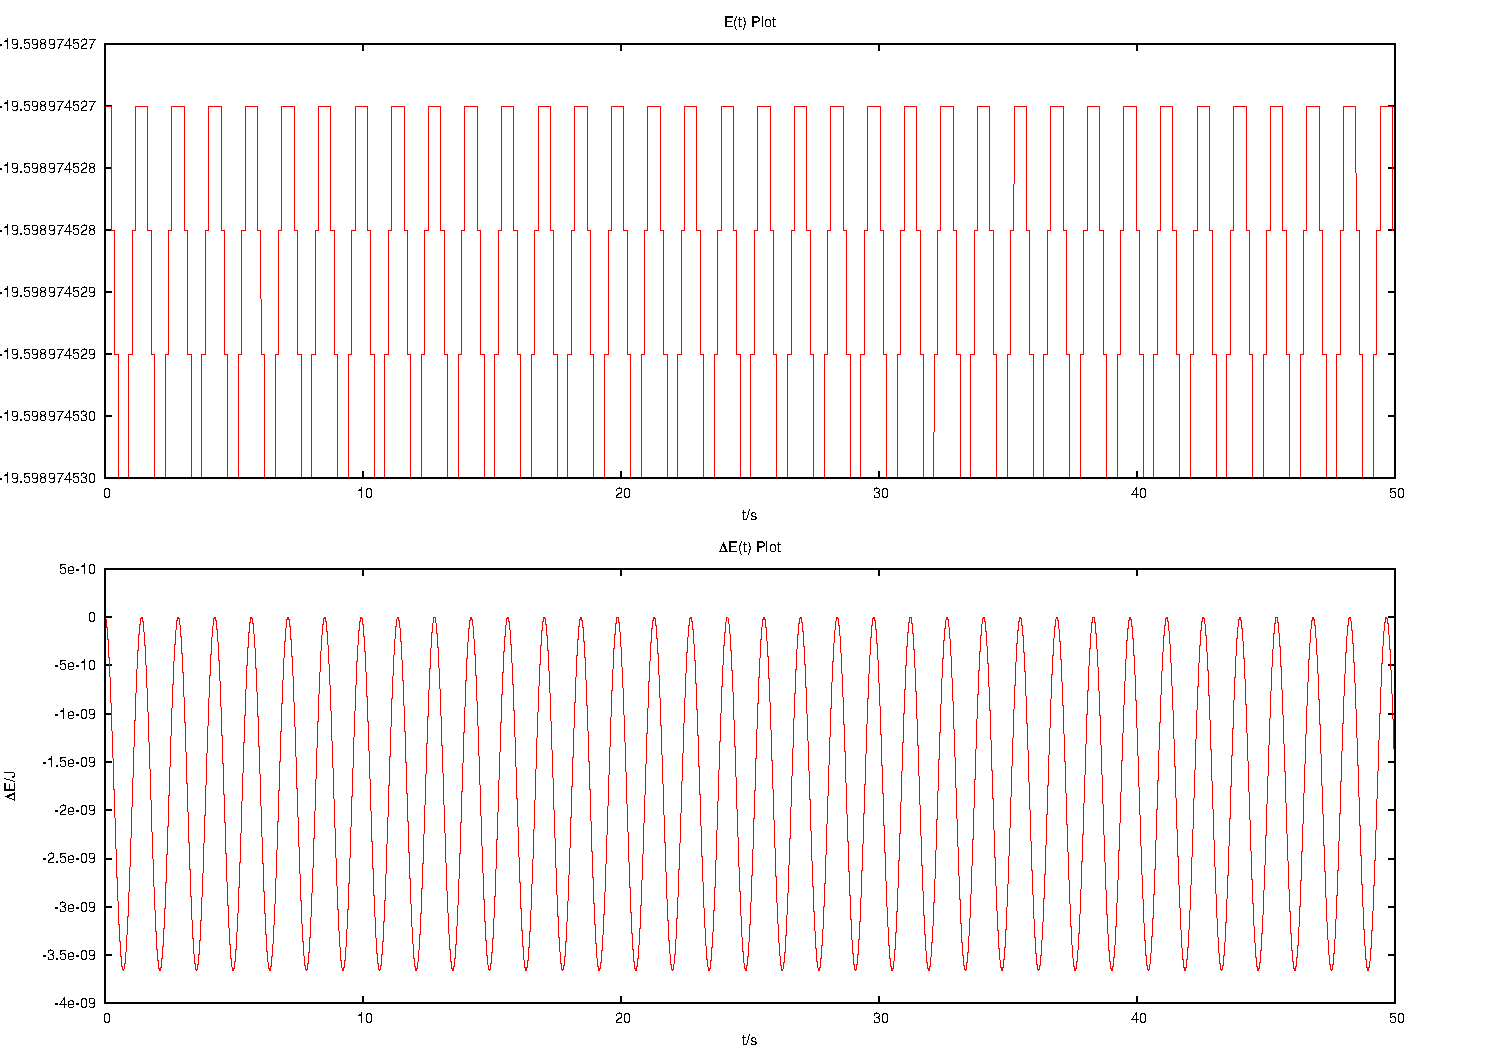
\includegraphics[width=0.9\textwidth]{./verletE.pdf}
\caption[Caption for LOF]{Verlet算法能量-时间曲线}
\label{fig:verletE}
\end{figure}
\begin{figure}[H]
\centering
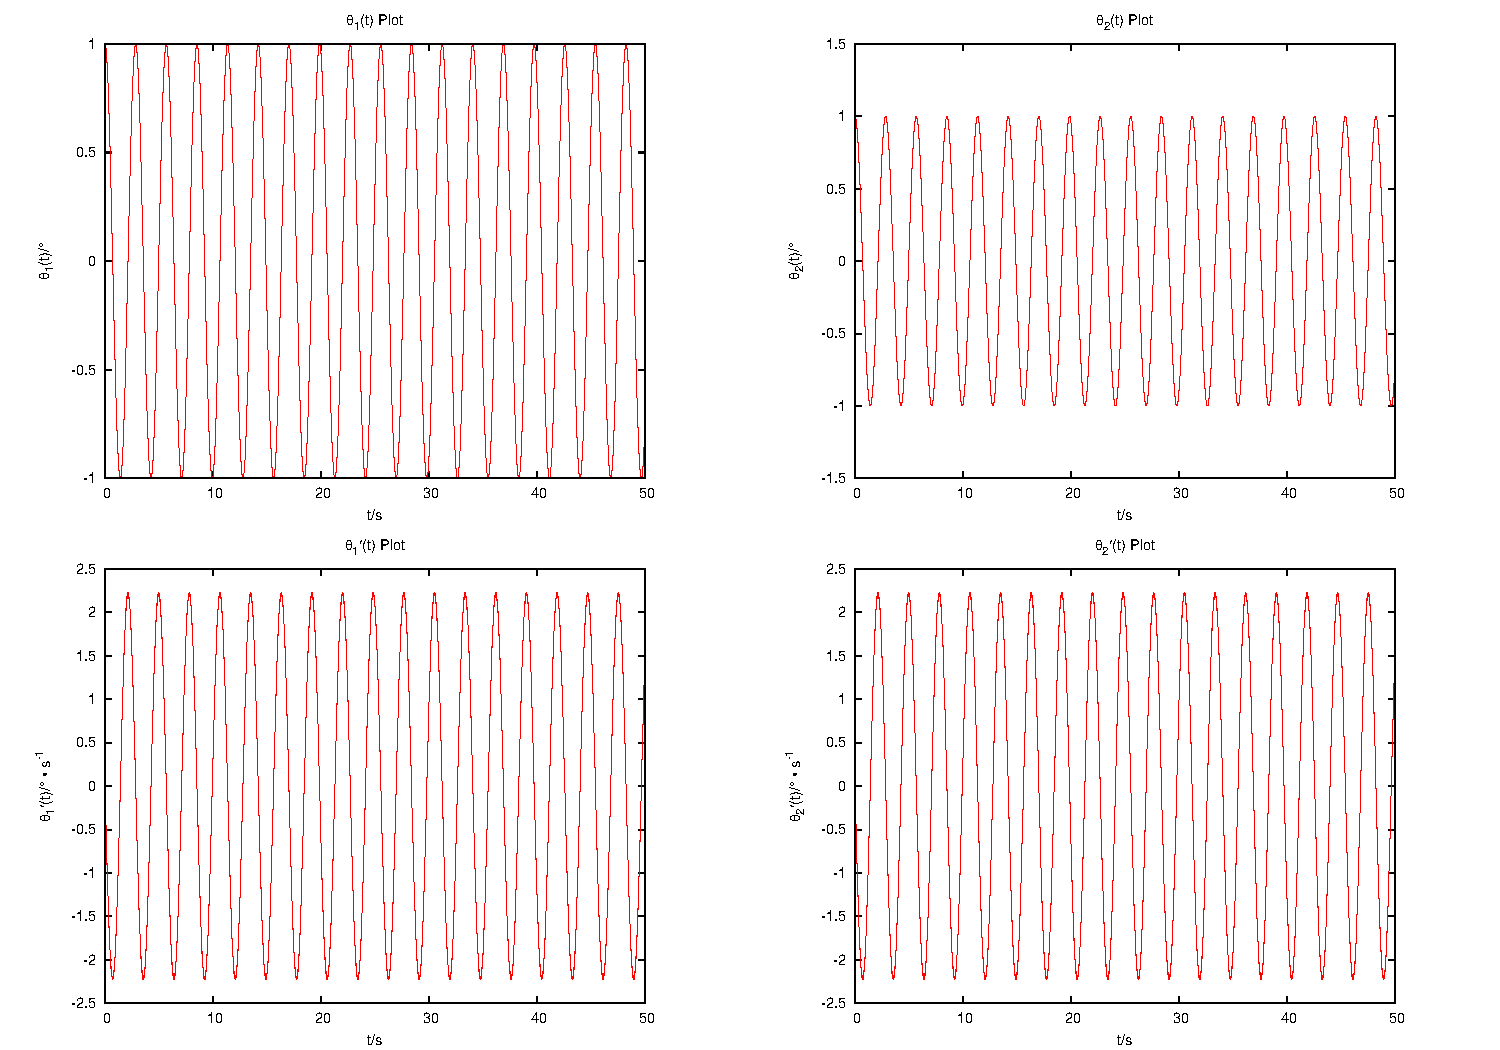
\includegraphics[width=0.8\textwidth]{./verletmove.pdf}
\caption[Caption for LOF]{Verlet算法运动-时间曲线}
\label{fig:verletmove}
\end{figure}
使用经典四阶Runge-Kutta算法模拟结果如图~\ref{fig:RKE_1}和图~\ref{fig:RKmove_1},其中,图~\ref{fig:RKE_1}为模拟过程中整个系统的能量变化情况。图~\ref{fig:RKmove_1}为系统角度和角速度的变化情况。
\begin{figure}[H]
\centering
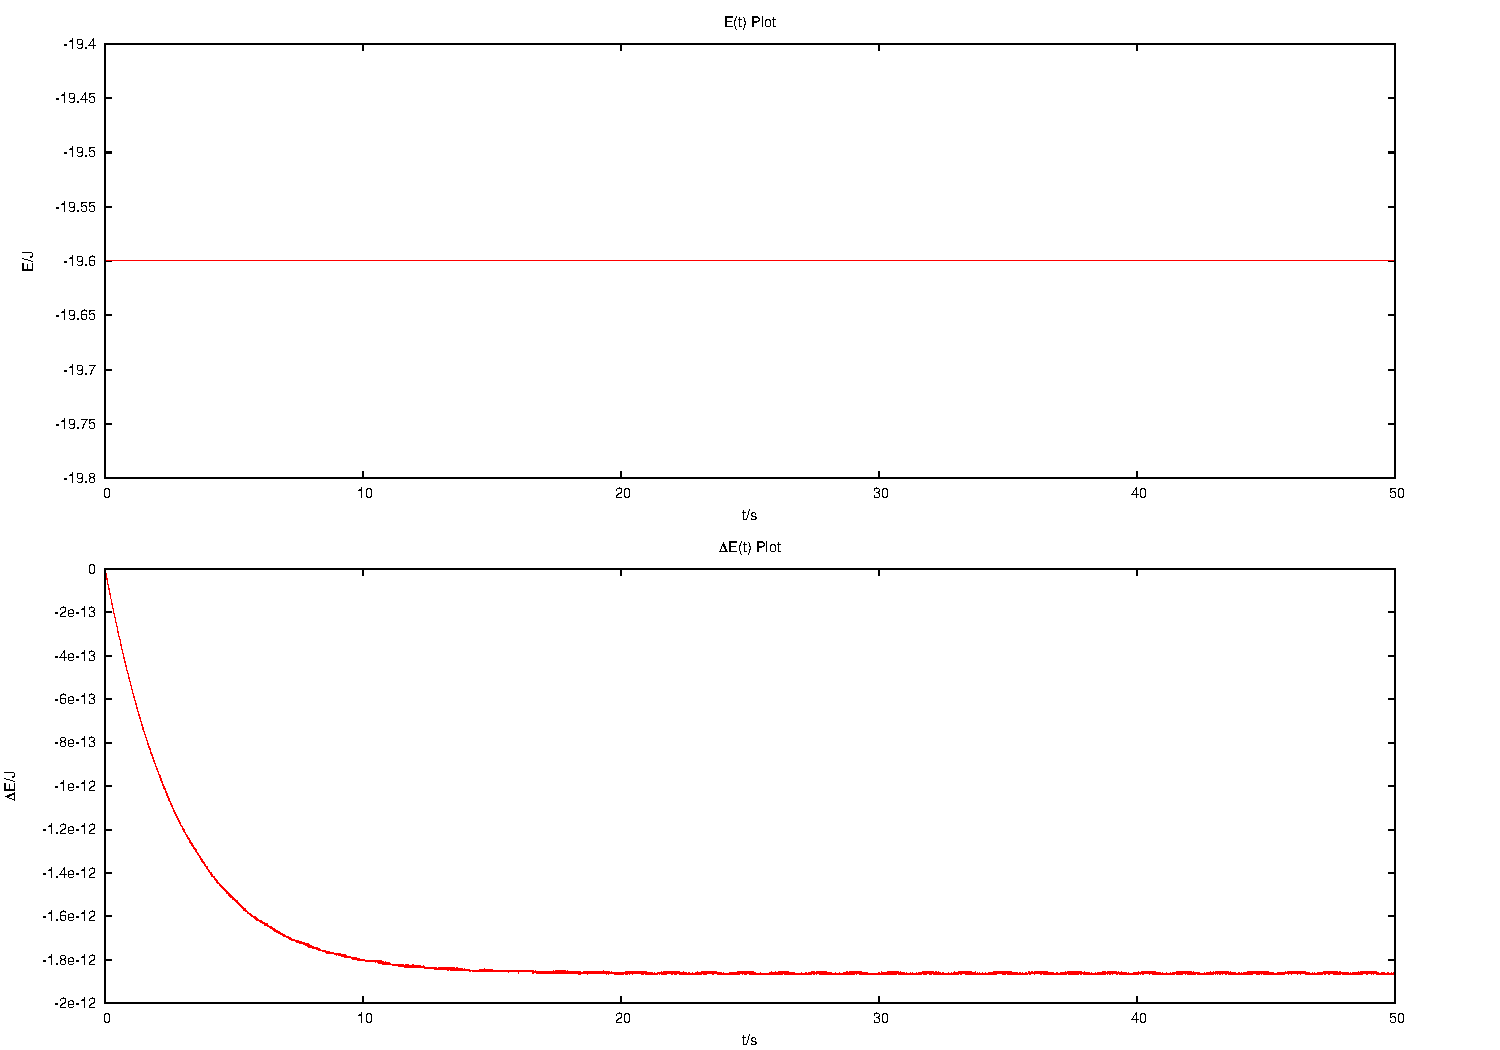
\includegraphics[width=0.8\textwidth]{./RKE_1.pdf}
\caption[Caption for LOF]{经典四阶Runge-Kutta算法能量-时间曲线}
\label{fig:RKE_1}
\end{figure}
\begin{figure}[H]
\centering
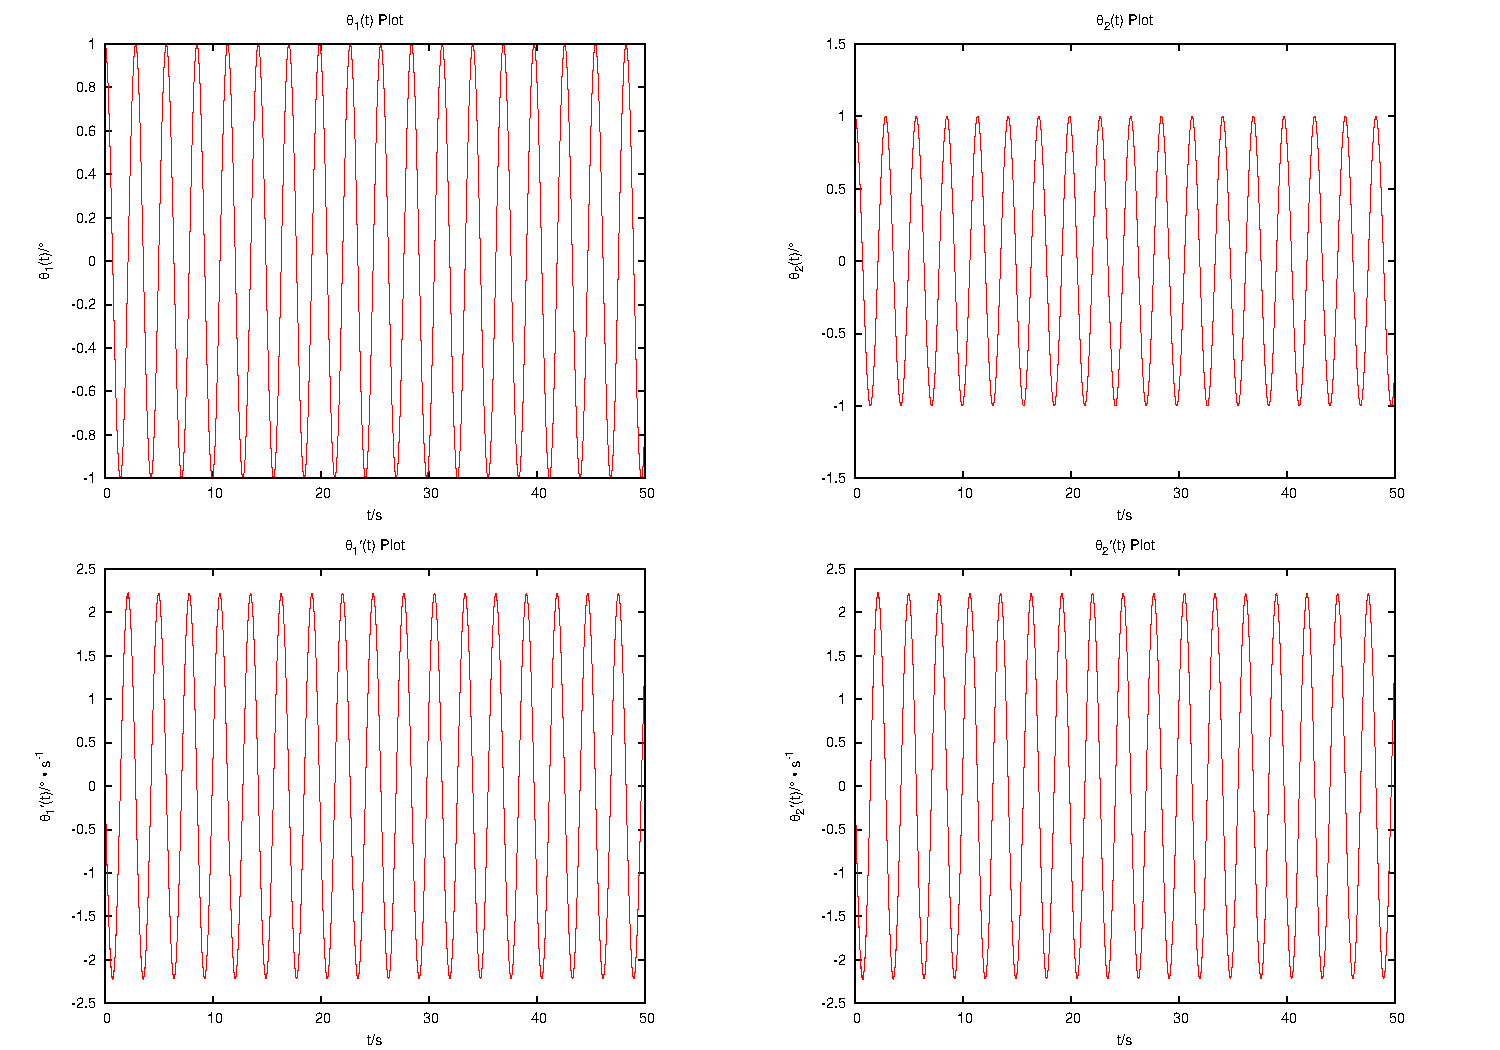
\includegraphics[width=0.8\textwidth]{./RKmove_1.pdf}
\caption[Caption for LOF]{经典四阶Runge-Kutta算法运动-时间曲线}
\label{fig:RKmove_1}
\end{figure}
从计算结果图可以简单估算出,模拟摆的周期为
\begin{equation}
	T=2.84~\mathrm{s} \notag
\end{equation}
同时,为了确定模拟摆的振荡函数的形式,对模拟结果的角度值(经典四阶Runge-Kutta算法结果)进行快速傅里叶变换(FFT),得到结果如图~\ref{fig:RKFFT_1}所示。
\begin{figure}[H]
\centering
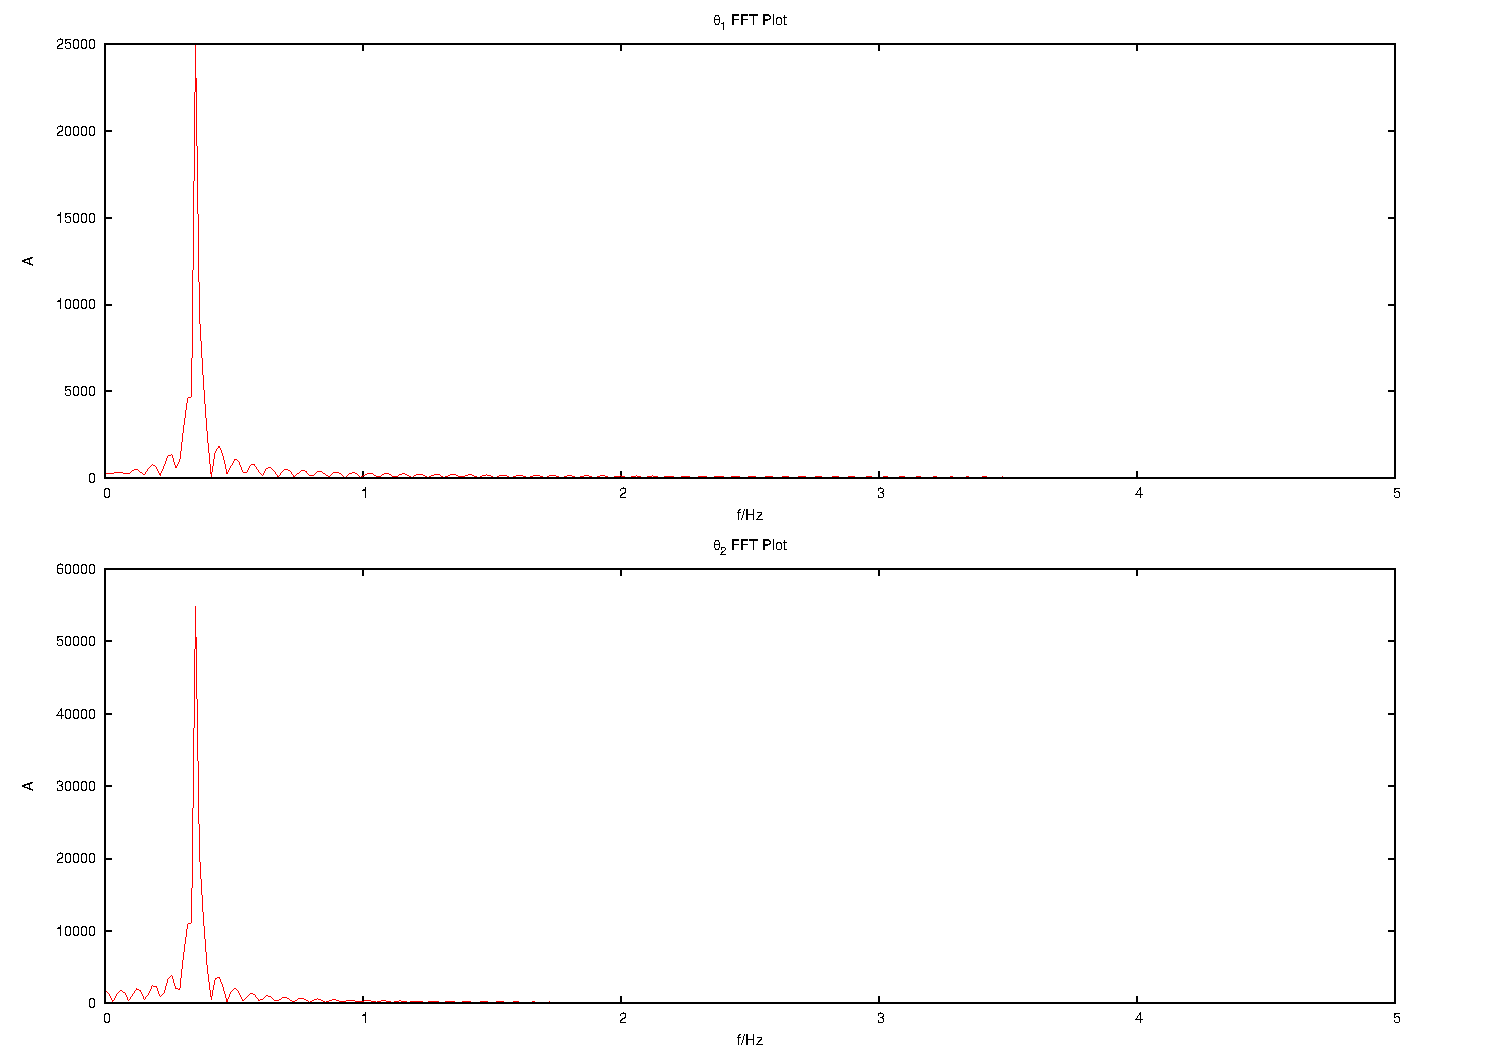
\includegraphics[width=0.7\textwidth]{./RKFFT_1.pdf}
\caption[Caption for LOF]{模拟摆运动的角度FFT曲线}
\label{fig:RKFFT_1}
\end{figure}
图\ref{fig:RKFFT_1}中,FFT曲线的形式为单峰模式,且峰的半高宽很窄。说明原函数的形式为三角函数形式。其中峰值在$f=0.351~\mathrm{Hz}$处,与理论值$f=0.3523~\mathrm{Hz}$很接近。

根据上述模拟结果,可以初步验证本文中设计的双杆复合摆的Verlet算法和经典Runge-Kutta算法是正确的。由于经典Runge-Kutta算法的精度更高,故可以根据经典Runge-Kutta算法的结果判断其他算法(如自适应时间步长算法)的正确性。

\subsection{典型双杆复合摆系统的运动特性}
典型双杆复合摆系统要求两段杆具有与摆锤可比的质量,两段杆的长度可比,且摆角不满足小角度条件。因此取初始条件为
\begin{equation}
	m_1=1~\mathrm{kg} ~,~ m_2=1~\mathrm{kg} ~,~ m_3=1~\mathrm{kg} ~,~ \theta_1=45^{\circ} ~,~ \theta_2=0^{\circ} \notag
\end{equation}
摆的运动-时间曲线如图~\ref{fig:move0}所示。
\begin{figure}[H]
\centering
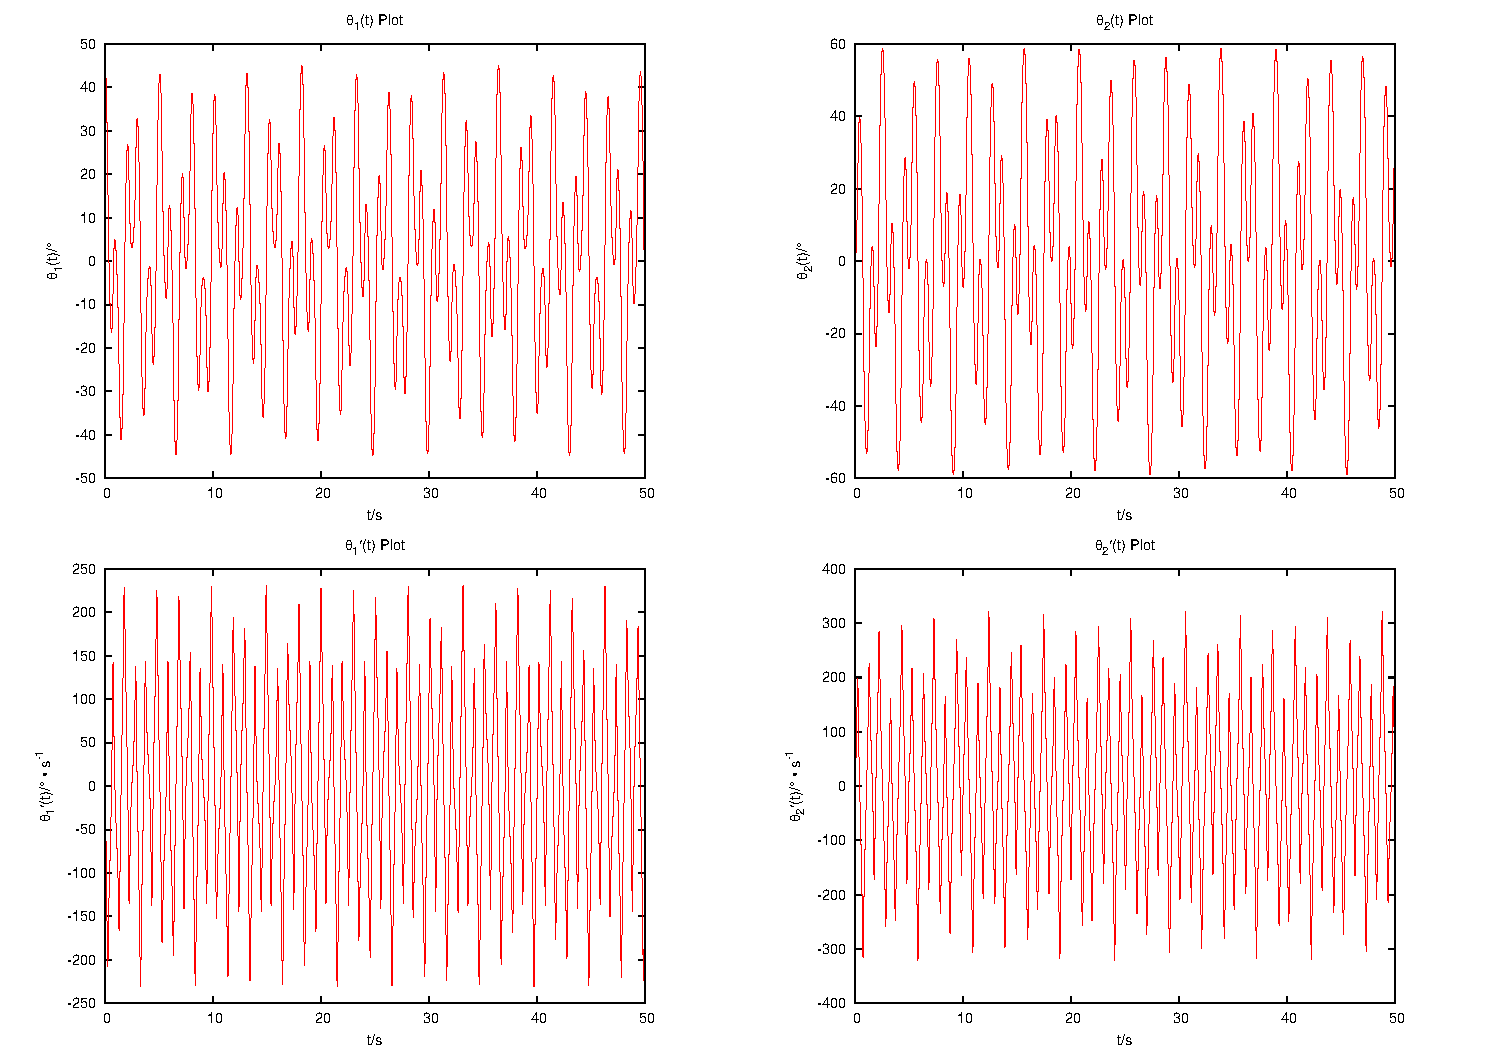
\includegraphics[width=0.9\textwidth]{./move0.pdf}
\caption[Caption for LOF]{双杆复合摆的运动-时间曲线}
\label{fig:move0}
\end{figure}
从图~\ref{fig:move0}可以看出,此时双杆摆的运动已经无法用初等函数表达,并且可能具有混沌的特性。为了更好的了解双杆摆此时的运动特性,对两个角度做快速傅里叶变换(FFT),得到如图~\ref{fig:FFT0}所示的结果。
\begin{figure}[H]
\centering
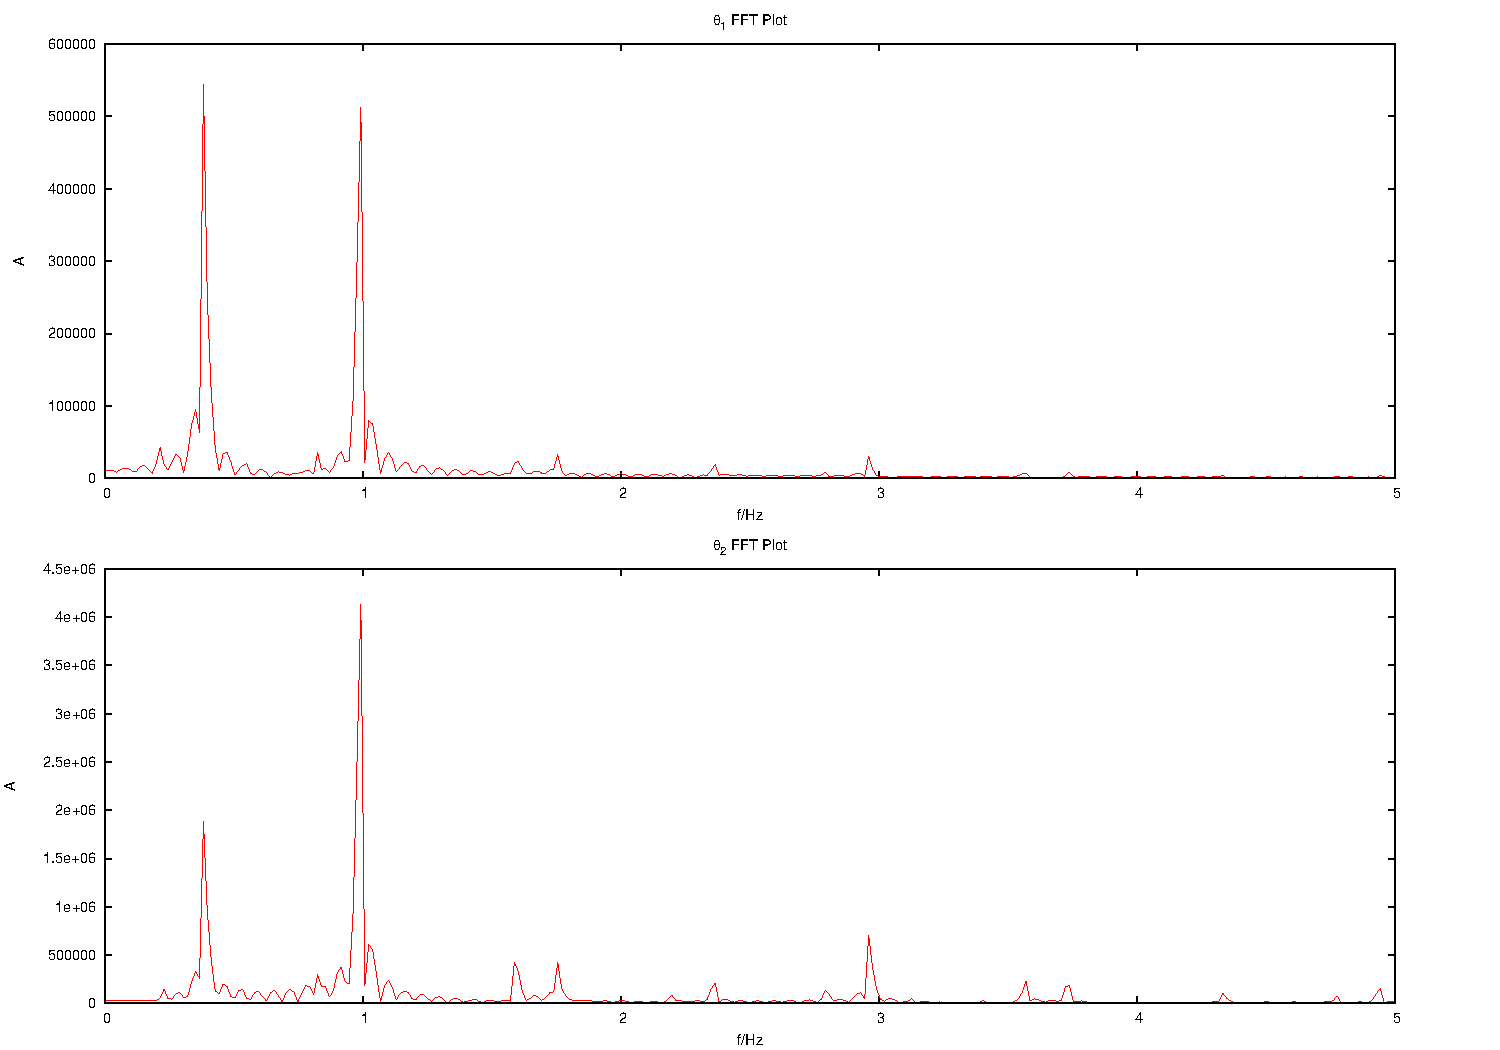
\includegraphics[width=0.7\textwidth]{./FFT0.pdf}
\caption[Caption for LOF]{双杆复合摆运动的FFT曲线}
\label{fig:FFT0}
\end{figure}
从FFT结果可以看出,运动出现了两个较强的振动频率,同时在高频段出现了高次谐波,类似于双摆球摆的两个本征频率。不同的是,双杆摆由于不是理想的双摆球摆,因此FFT结果中在本征频率附近出现了大量杂频,同时本征频率的峰也有所展宽。

\subsection{Verlet算法与经典Runge-Kutta算法精度比较}
算法简介中已经指出,经典Runge-Kutta算法为五阶收敛,而Verlet算法为二阶收敛,因此从收敛性的角度考虑,经典Runge-Kutta算法要好于Verlet算法。

显然,无阻尼的双杆复合摆系统为机械能守恒系统,因此,可以通过比较系统机械能的变化来判断算法的收敛性。模拟中,取初始条件为
\begin{equation}
	m_1=1~\mathrm{kg} ~,~ m_2=1~\mathrm{kg} ~,~ m_3=1~\mathrm{kg} ~,~ \theta_1=45^{\circ} ~,~ \theta_2=0^{\circ} \notag
\end{equation}
两种算法模拟的能量-时间曲线如图~\ref{fig:verletE_2}和图~\ref{fig:RKE_2}所示。
\begin{figure}[H]
\centering
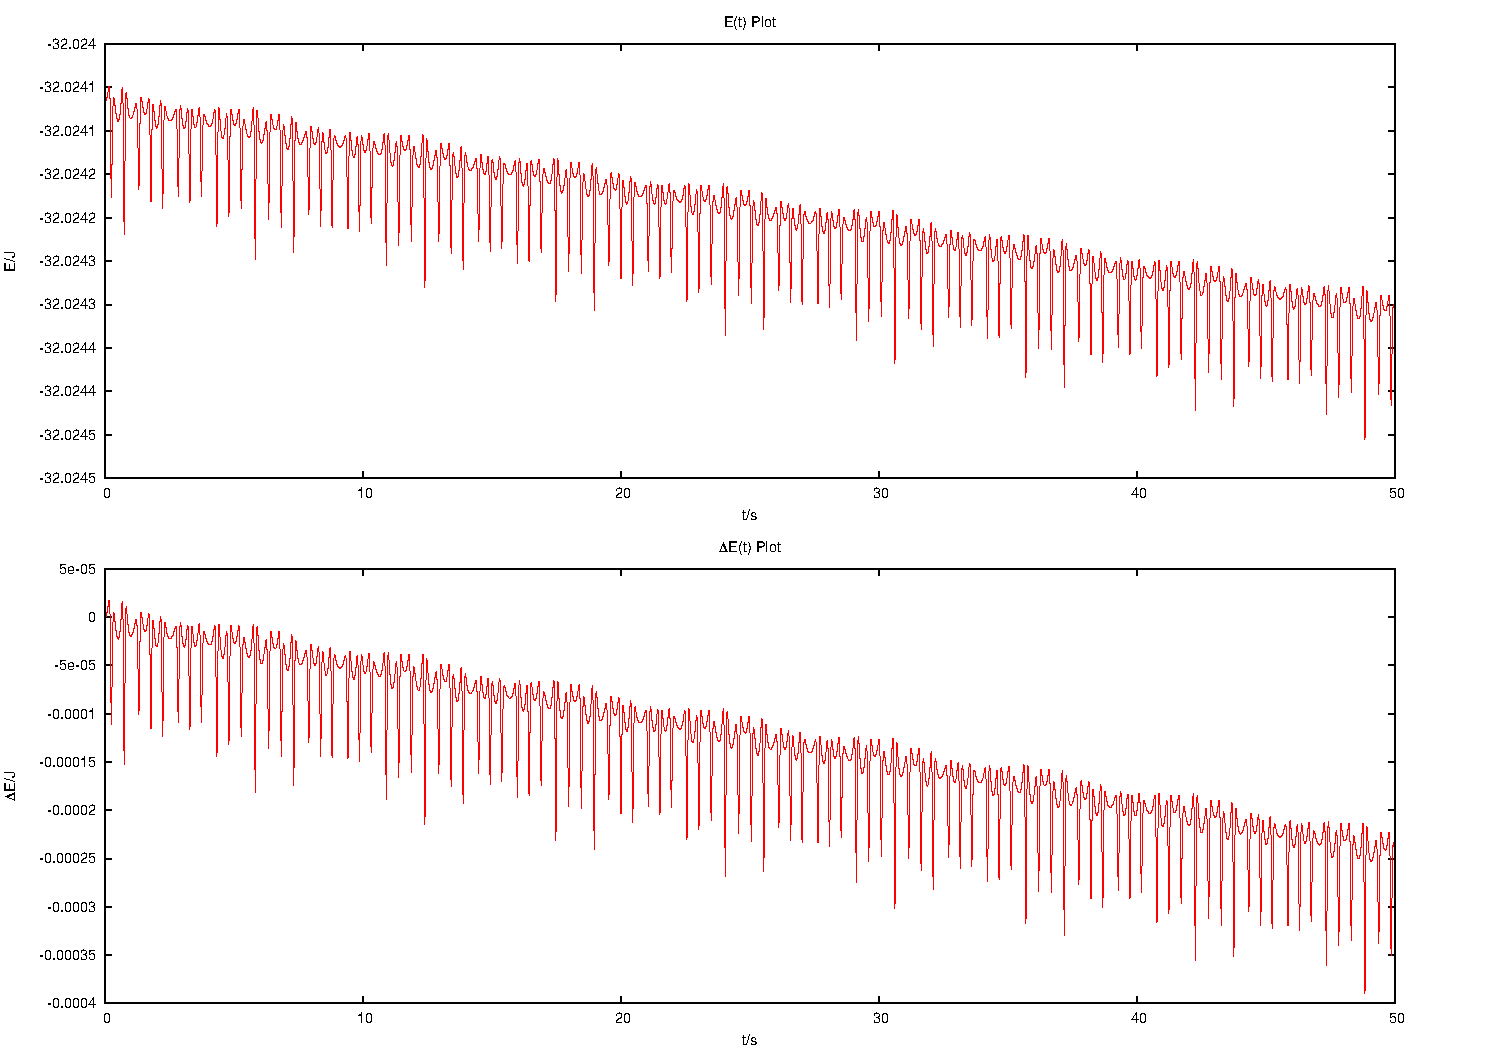
\includegraphics[width=0.8\textwidth]{./verletE_2.pdf}
\caption[Caption for LOF]{Verlet算法能量-时间曲线}
\label{fig:verletE_2}
\end{figure}
\begin{figure}[H]
\centering
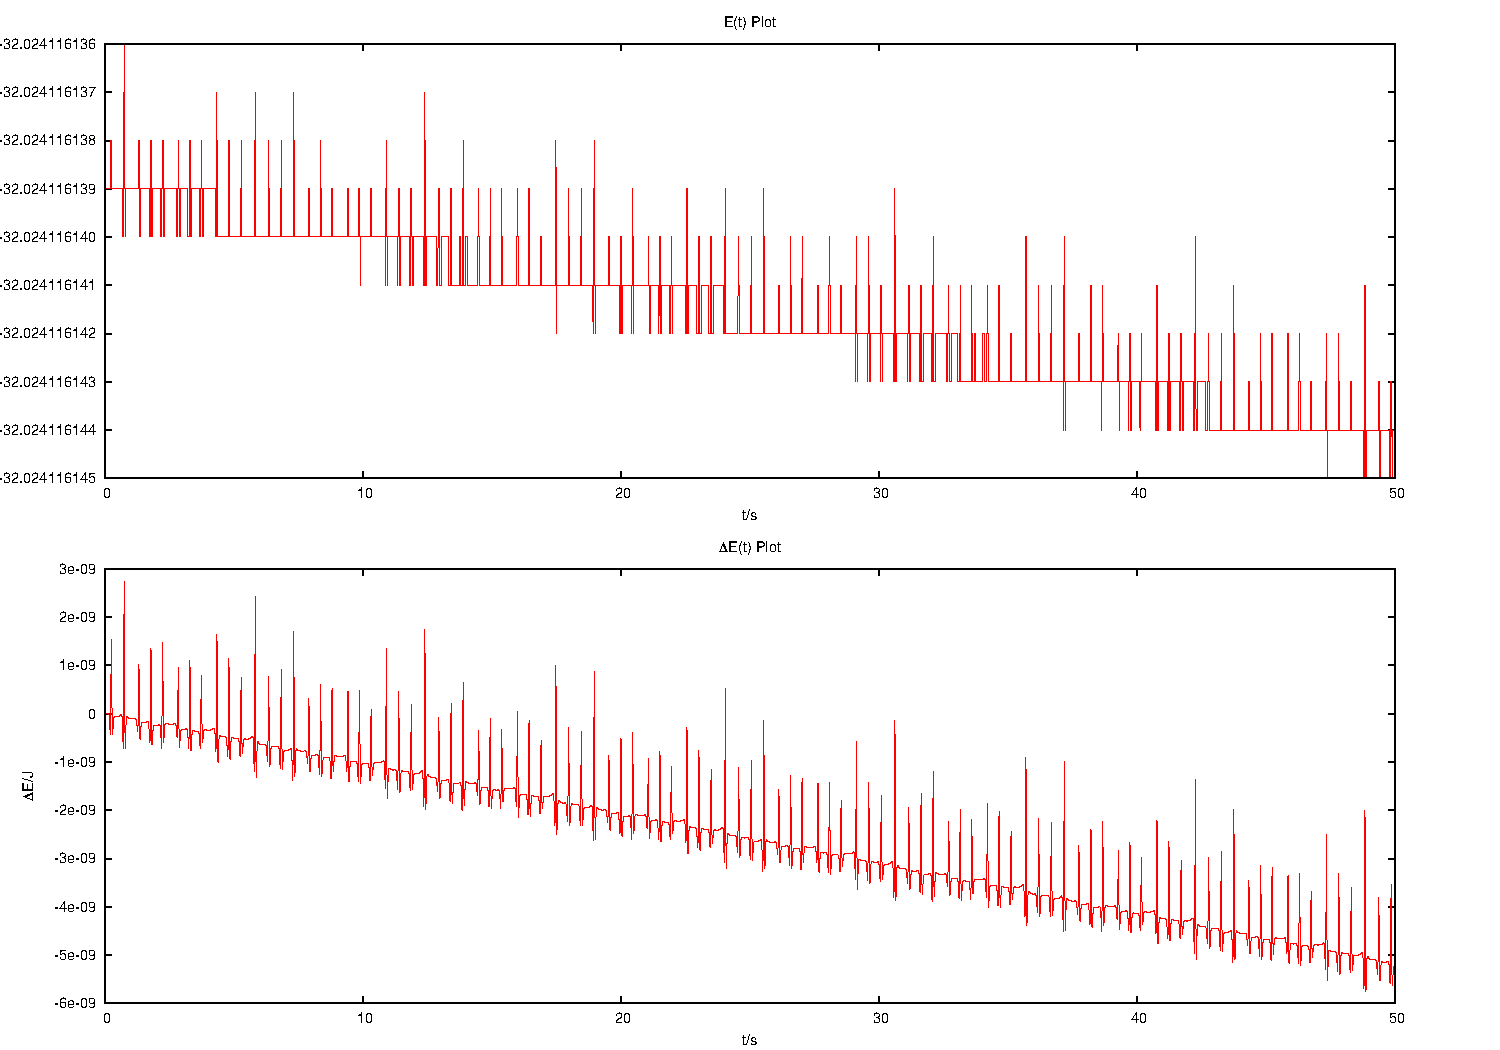
\includegraphics[width=0.8\textwidth]{./RKE_2.pdf}
\caption[Caption for LOF]{经典四阶Runge-Kutta算法能量-时间曲线}
\label{fig:RKE_2}
\end{figure}
从模拟结果可以看出,
\begin{enumerate}
	\item Verlet算法的能量误差的绝对值要大于经典Runge-Kutta算法4$\sim$5个数量级;
	\item Verlet算法的能量存在明显的累积误差,而经典Runge-Kutta算法的累积误差相对小4$~\sim$5个数量级。
\end{enumerate}

根据上述结果可以得出结论,经典Runge-Kutta算法的计算精度要明显高于Verlet算法。

\subsection{经典Runge-Kutta算法与自适应时间步长算法的比较}
根据之前的论述可知,自适应时间步长算法的优势在于对于误差较低的初始值,可以提高步长从而降低计算时间,对于误差较高的初始值,可以缩短步长提升计算精度,因此自适应时间步长算法对于不同初始条件的自适应性要好于固定步长的经典Runge-Kutta算法。

若取初始条件为
\begin{equation}
	m_1=1~\mathrm{kg} ~,~ m_2=1~\mathrm{kg} ~,~ m_3=1~\mathrm{kg} ~,~ \theta_1=45^{\circ} ~,~ \theta_2=0^{\circ} ~,~ t_{total}=500 ~\mathrm{s} \notag
\end{equation}
算法的默认时间步长为
\begin{equation}
	dt=1.0 ~\mathrm{ms}\notag
\end{equation}
自适应时间步长算法的期望误差值
\begin{equation}
	\Delta_0=1.0\times 10^{-10} ~\mathrm{J}\notag
\end{equation}
经典Runge-Kutta算法与自适应时间步长算法的计算时间(典型值)分别为
\begin{align}
	T_{RK}=&2.458842 ~\mathrm{s}\notag \\
	T_{Adaptive}=&1.757877 ~\mathrm{s}\notag
\end{align}
两种算法的能量-时间曲线如图~\ref{fig:RKE_3}和图~\ref{fig:RKAE_3}
\begin{figure}[H]
\centering
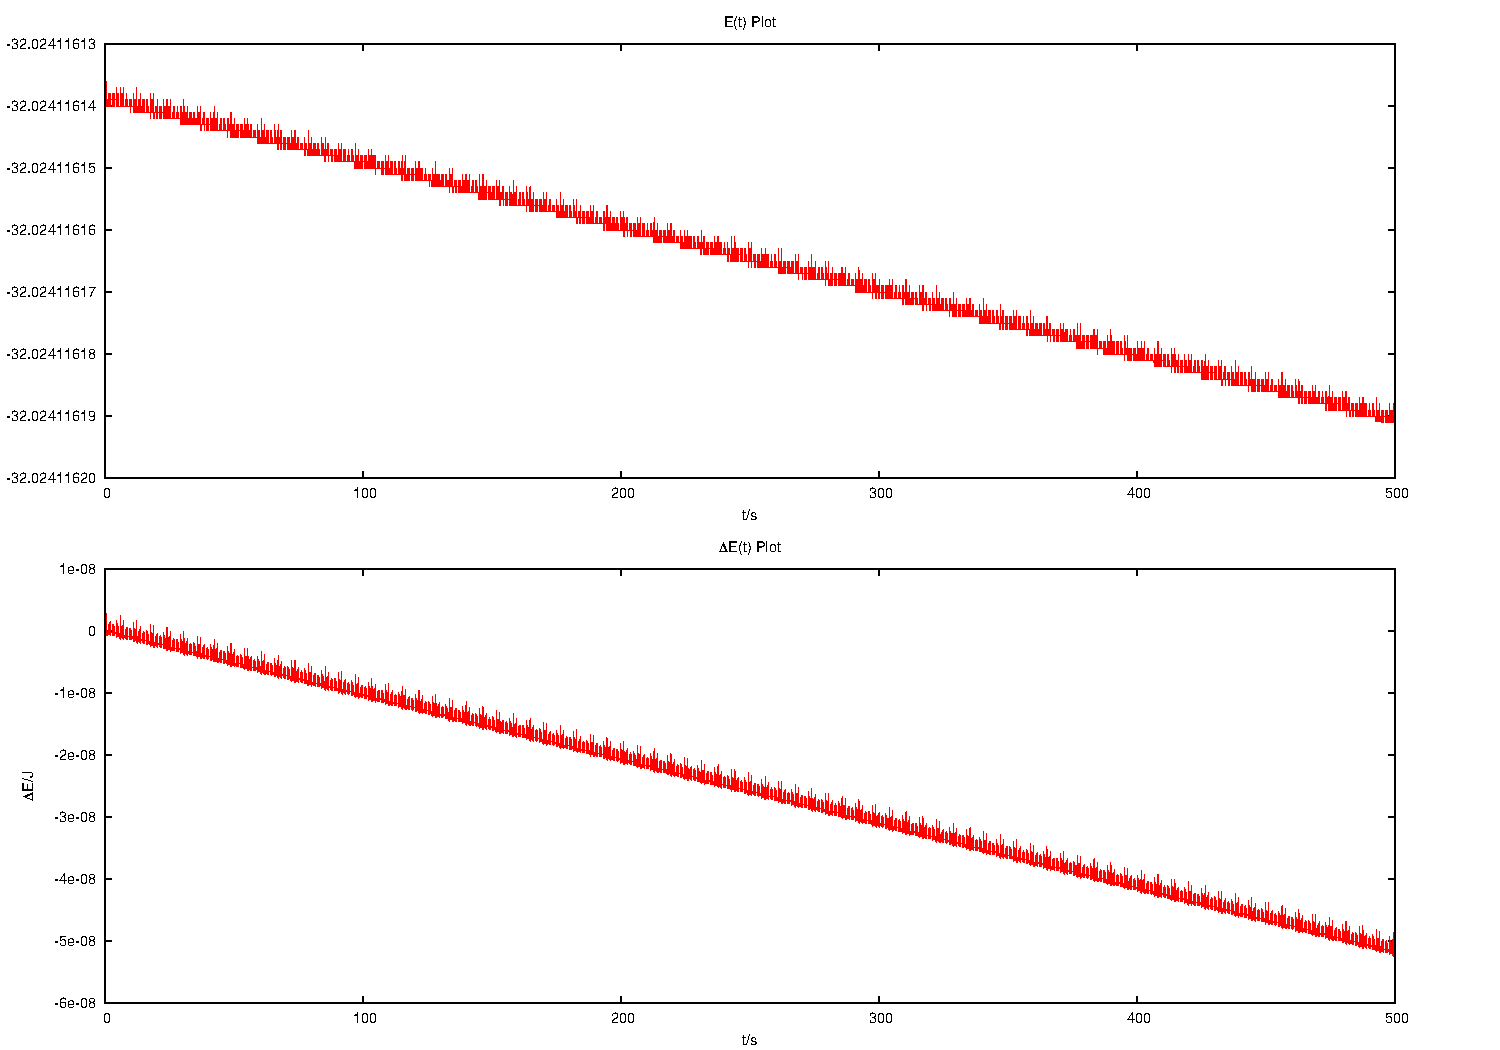
\includegraphics[width=0.7\textwidth]{./RKE_3.pdf}
\caption[Caption for LOF]{经典四阶Runge-Kutta算法能量-时间曲线}
\label{fig:RKE_3}
\end{figure}
\begin{figure}[H]
\centering
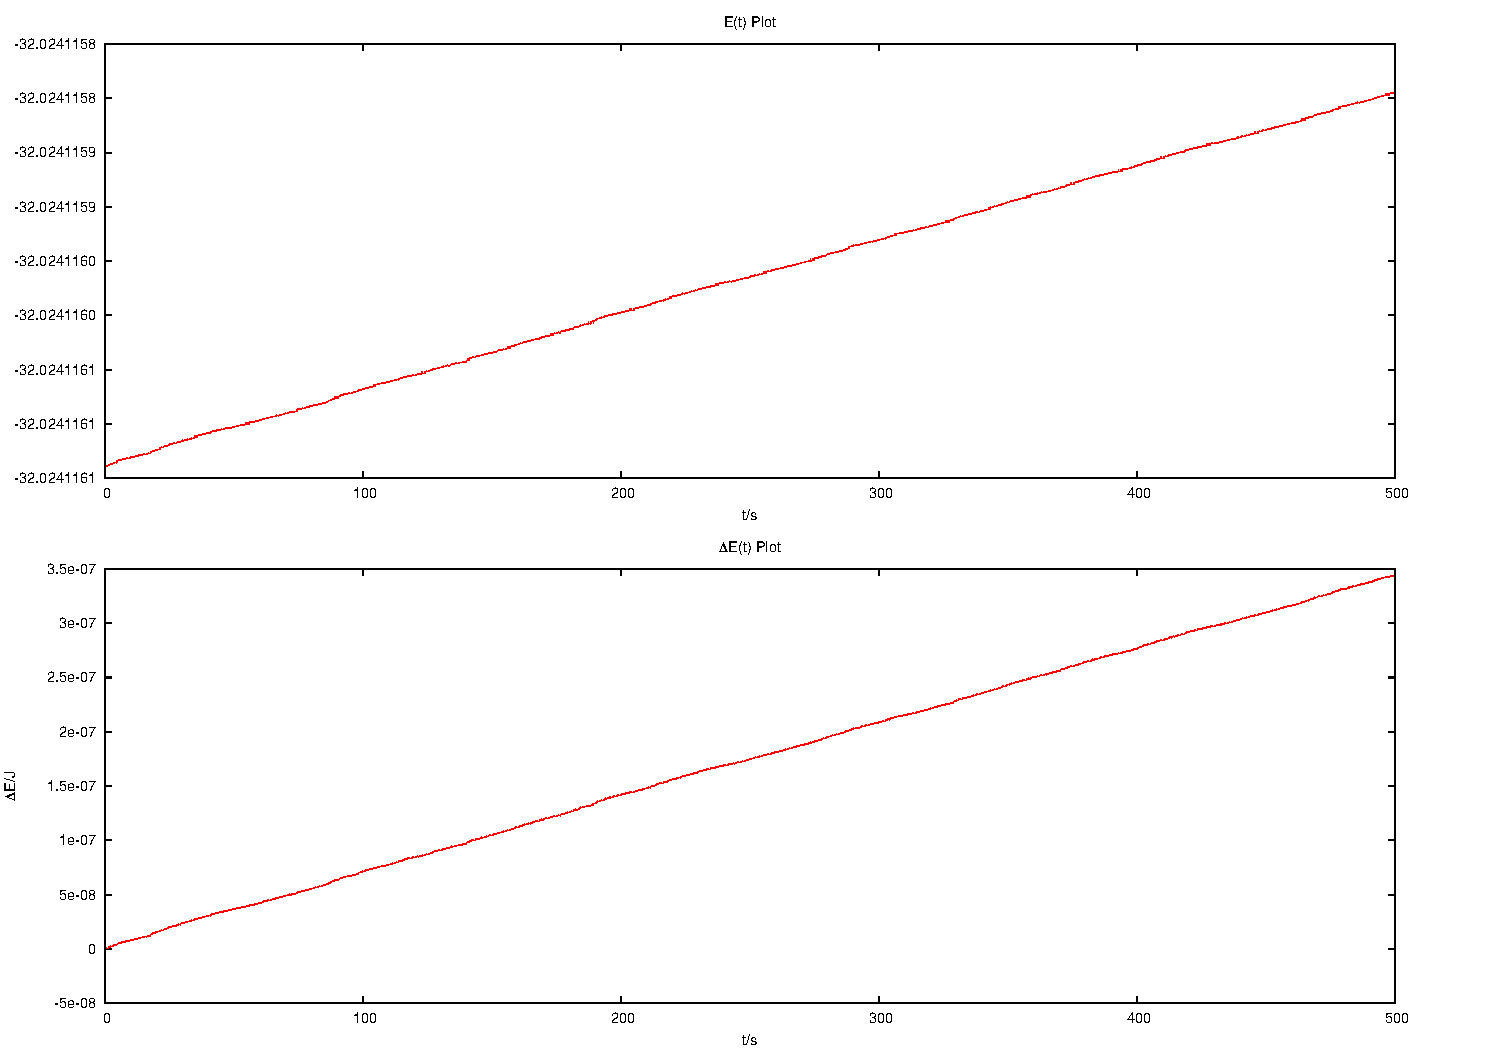
\includegraphics[width=0.7\textwidth]{./RKAE_3.pdf}
\caption[Caption for LOF]{自适应时间步长算法能量-时间曲线}
\label{fig:RKAE_3}
\end{figure}

多次计算后发现,自适应时间步长算法的计算时间均在1.7s附近,小于经典Runge-Kutta算法的2.4s的典型值,说明自适应时间步长算法的计算速度更快。经程序统计,自适应时间步长算法的平均时间步长(典型值)为
\begin{equation}
	dt=2.468002 ~\mathrm{ms} > dt_0=1.0 ~\mathrm{ms}\notag
\end{equation}
在整个计算过程中,自适应时间步长算法的时间步长变化如图~\ref{fig:RKAdt_3}所示。
\begin{figure}[H]
\centering
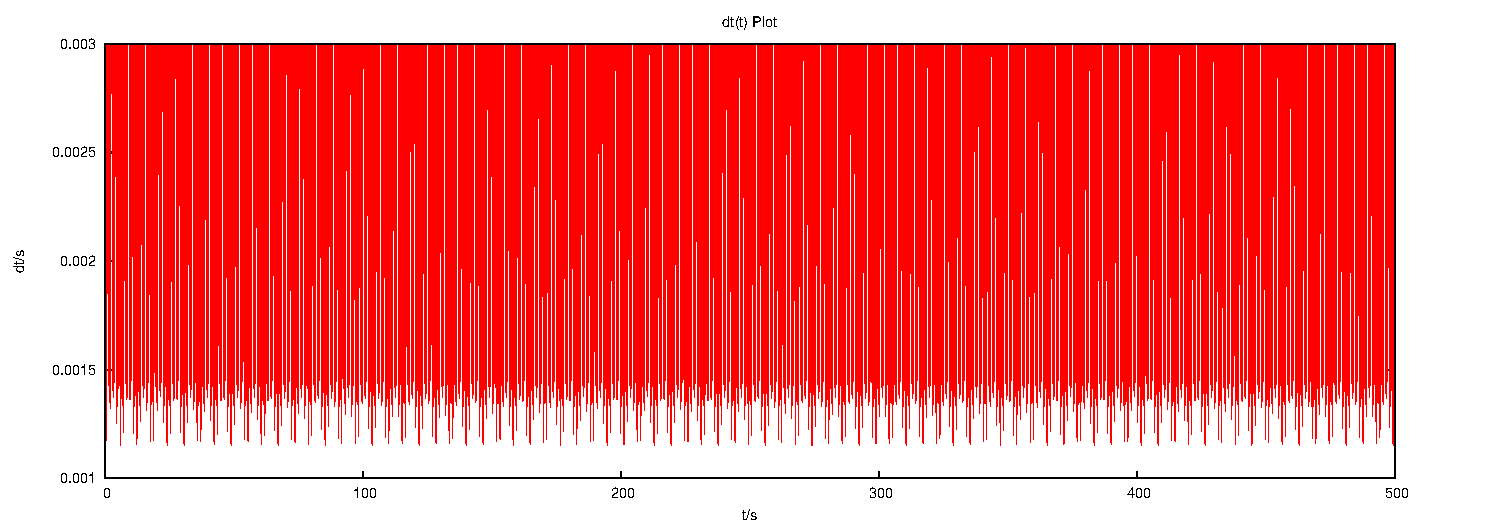
\includegraphics[width=0.9\textwidth]{./RKAdt_3.pdf}
\caption[Caption for LOF]{自适应时间步长算法时间步长-时间曲线}
\label{fig:RKAdt_3}
\end{figure}

从两种算法的误差来看,在上述初始条件情况下,自适应时间步长算法的计算精度要低于经典Runge-Kutta算法,这是由于自适应时间步长算法的计算精度是由程序中设定的期望误差值$\Delta_0$决定,而不由运动过程决定。同时自适应时间步长算法不会因为不同的运动状态而导致误差的大幅波动,下面取一种极端的情况来说明自适应时间步长算法的这种性质。

取初始条件为
\begin{equation}
	m_1=1~\mathrm{kg} ~,~ m_2=1~\mathrm{kg} ~,~ m_3=1~\mathrm{kg} ~,~ \theta_1=180^{\circ} ~,~ \theta_2=179^{\circ} ~,~ t_{total}=500 ~\mathrm{s}\notag
\end{equation}
算法的默认时间步长为
\begin{equation}
	dt=1.0 ~\mathrm{ms}\notag
\end{equation}
自适应时间步长算法的期望误差值
\begin{equation}
	\Delta_0=1.0\times 10^{-10} ~\mathrm{J}\notag
\end{equation}
经典Runge-Kutta算法与自适应时间步长算法的计算时间(典型值)分别为
\begin{align}
	T_{RK}=&2.480281 ~\mathrm{s} \notag \\
	T_{Adaptive}=&3.097844 ~\mathrm{s}\notag
\end{align}
两种算法的能量-时间曲线如图~\ref{fig:RKE_4}和图~\ref{fig:RKAE_4}
\begin{figure}[H]
\centering
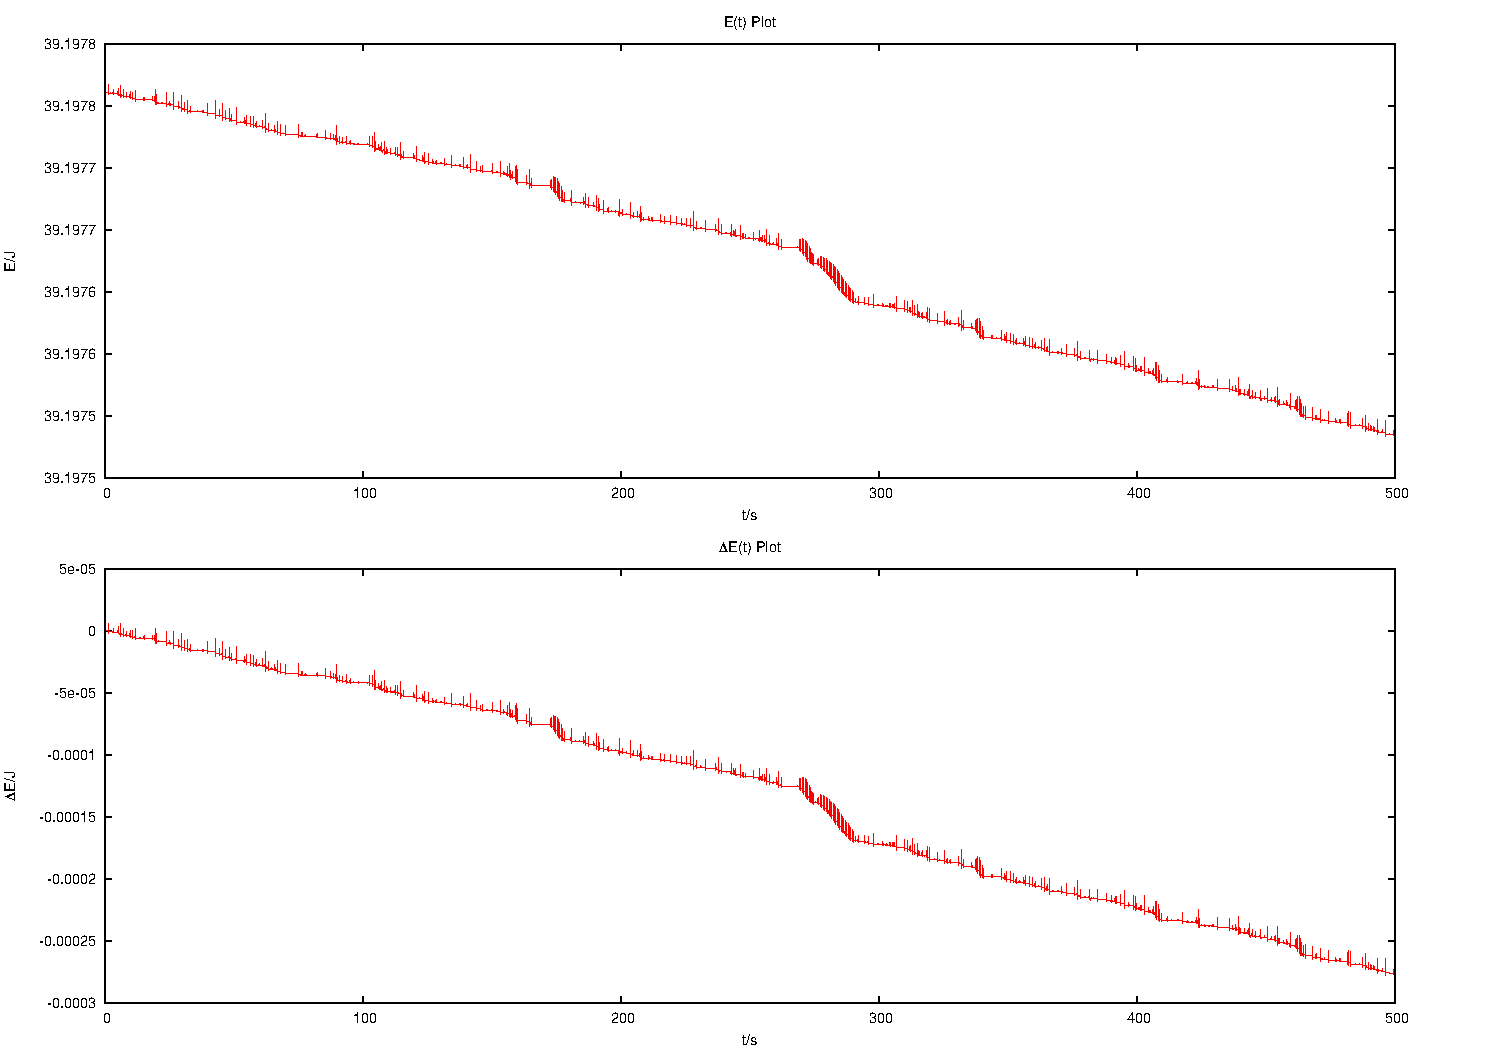
\includegraphics[width=0.8\textwidth]{./RKE_4.pdf}
\caption[Caption for LOF]{经典四阶Runge-Kutta算法能量-时间曲线}
\label{fig:RKE_4}
\end{figure}
\begin{figure}[H]
\centering
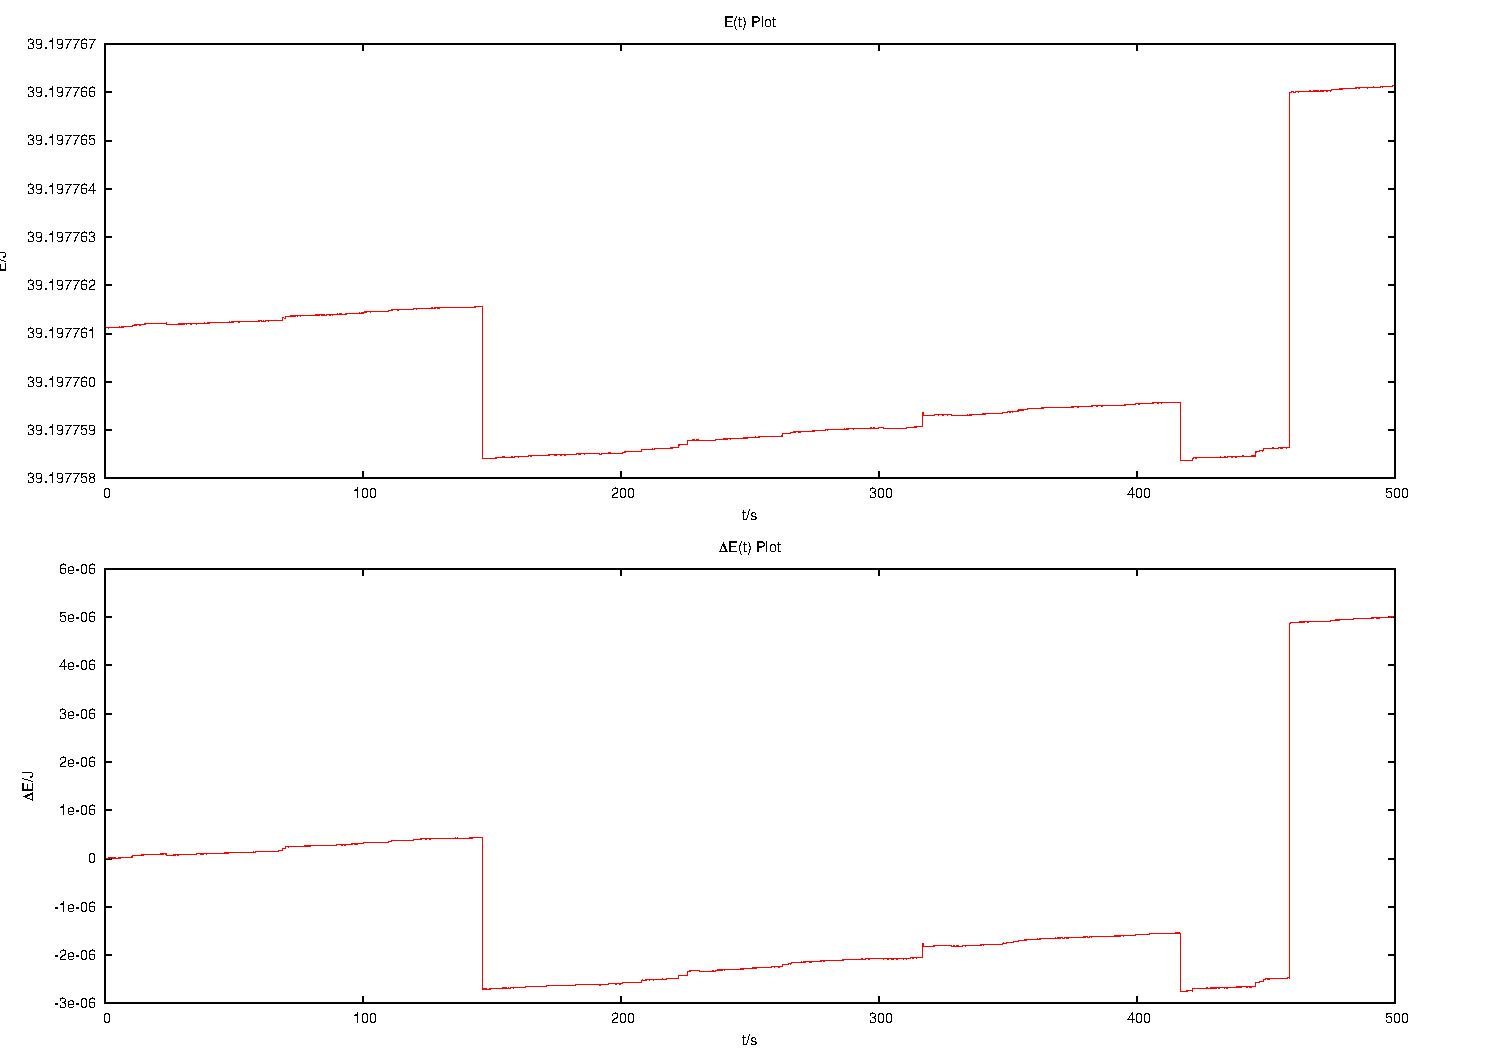
\includegraphics[width=0.8\textwidth]{./RKAE_4.pdf}
\caption[Caption for LOF]{自适应时间步长算法能量-时间曲线}
\label{fig:RKAE_4}
\end{figure}

更改初始条件后,自适应时间步长算法的计算时间均在3.1s附近,大于经典Runge-Kutta算法的2.4s的典型值。实际上经典Runge-Kutta算法的计算时间是不变的,因为经典Runge-Kutta算法的时间步长一定导致计算总步数不因问题初始条件不同而改变,而自适应时间步长算法会因为初值条件不同而改变时间步长,进而导致计算总步数不定,最终影响程序执行时间。经程序统计,自适应时间步长算法的平均时间步长(典型值)为
\begin{equation}
	dt=1.380723 ~\mathrm{ms} > dt_0=1.0 ~\mathrm{ms} \notag
\end{equation}
在整个计算过程中,自适应时间步长算法的时间步长变化如图~\ref{fig:RKAdt_4}所示。
\begin{figure}[H]
\centering
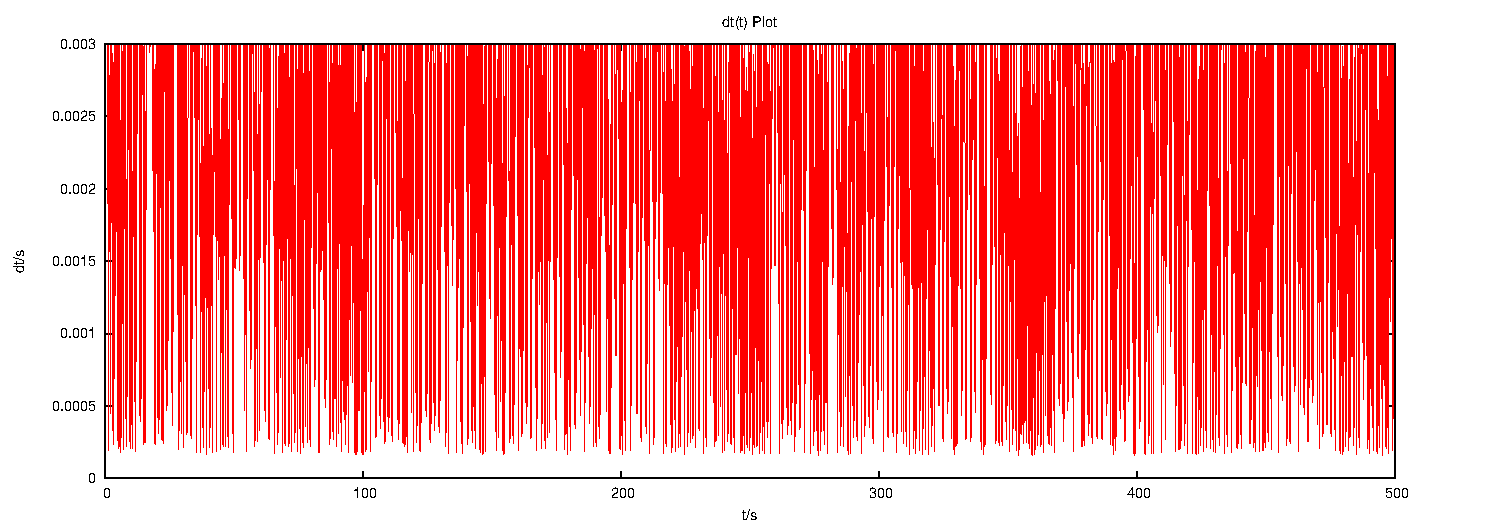
\includegraphics[width=0.9\textwidth]{./RKAdt_4.pdf}
\caption[Caption for LOF]{自适应时间步长算法时间步长-时间曲线}
\label{fig:RKAdt_4}
\end{figure}

此时,自适应时间步长算法的计算精度与之前相比几乎没有变化,仅仅因为计算过程中的偶然出现的极端初值条件导致一定程度的跳变,但仍在计算精度内。而经典Runge-Kutta算法的计算误差则增大了超过4个量级。并且,仔细观察可以发现,经典Runge-Kutta算法出现了明显的累积误差。

上述对比说明了自适应时间步长算法对于计算精度和计算时间的自动平衡和避免累积误差的能力,体现了自适应性的优势,即无需人为修改参数,算法可以根据不同时刻的初值条件自动取得计算精度和计算时间的最佳平衡(通过调整期望误差参数),同时减少累积误差,非常适用于长时间的复杂变化系统的数值模拟。

\section{有空气阻力的双杆复合摆系统模拟特性}
若按照公式(\ref{eq:force1})及方程(\ref{eq:af11})~(\ref{eq:af12})~(\ref{eq:af21})~(\ref{eq:af22})所示结构,在模拟程序中加入空气阻力的影响。

若取初始条件为
\begin{equation}
	m_1=1~\mathrm{kg} ~,~ m_2=1~\mathrm{kg} ~,~ m_3=1~\mathrm{kg} ~,~ \theta_1=45^{\circ} ~,~ \theta_2=0^{\circ} ~,~ t_{total}=500 ~\mathrm{s} \notag
\end{equation}
算法的默认时间步长为
\begin{equation}
	dt=1.0 ~\mathrm{ms} \notag
\end{equation}
采用经典Runge-Kutta法进行计算。

取不同的空气阻尼系数$\mu$,可得双杆摆的运动和能量变化曲线如图~\ref{fig:rss1E}、图~\ref{fig:rss1move}及图~\ref{fig:rss2E}、图~\ref{fig:rss2move}所示。
\begin{figure}[H]
\centering
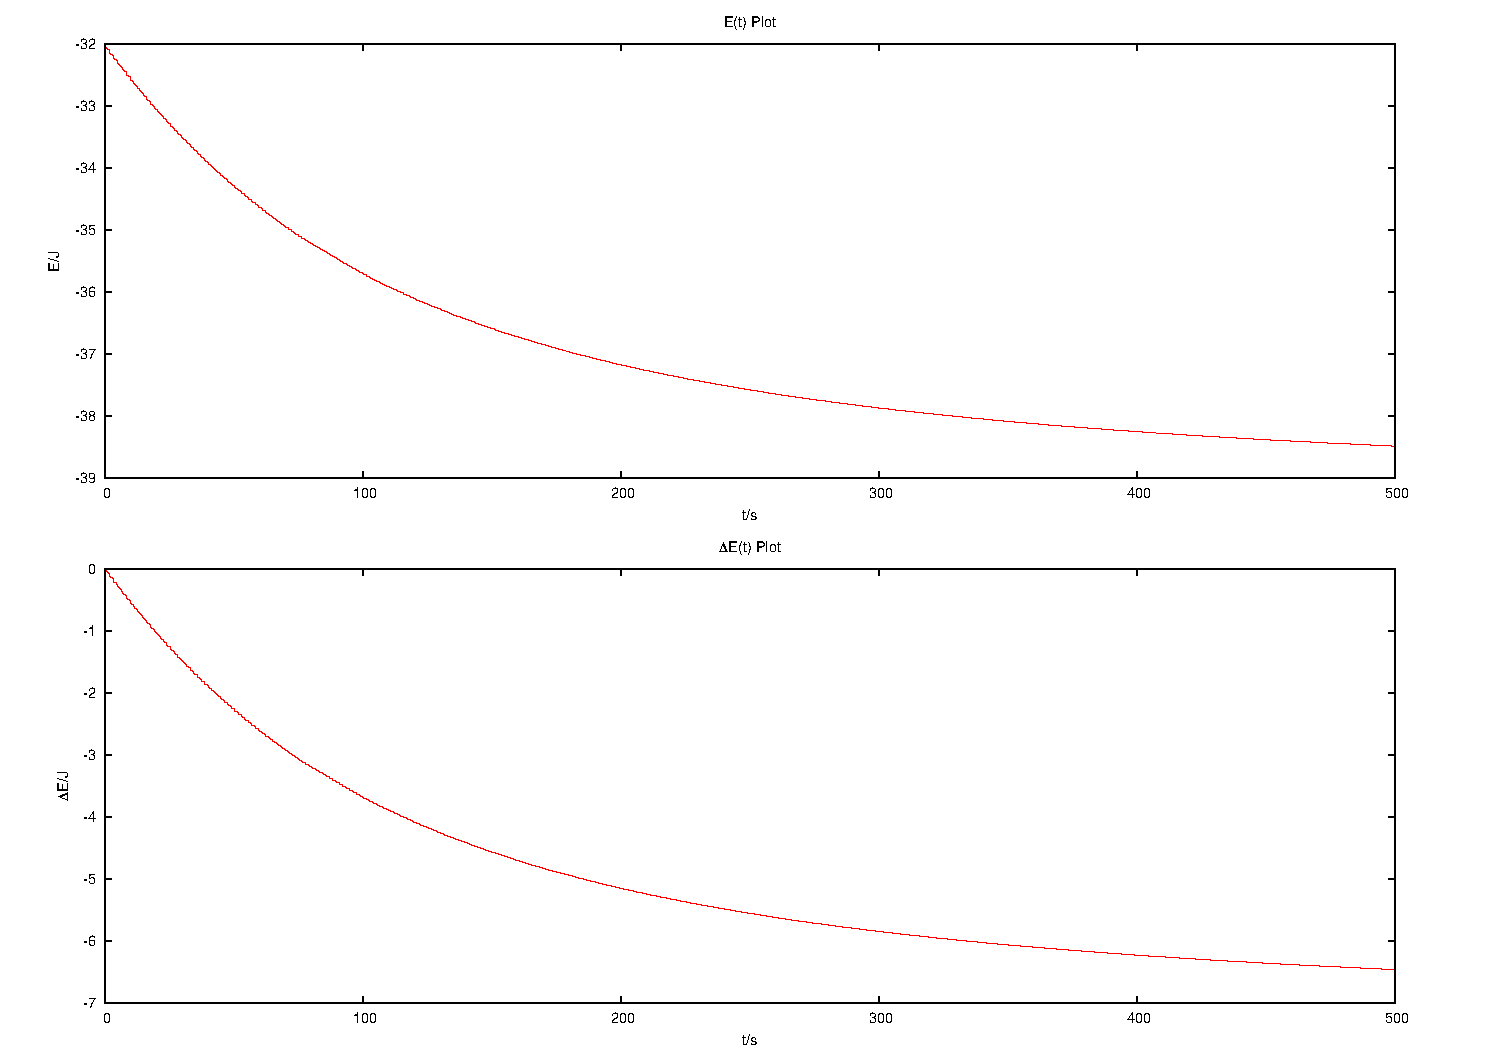
\includegraphics[width=0.8\textwidth]{./rss1E.pdf}
\caption[Caption for LOF]{空气阻尼系数$\mu=0.01$时的能量-时间曲线}
\label{fig:rss1E}
\end{figure}
\begin{figure}[H]
\centering
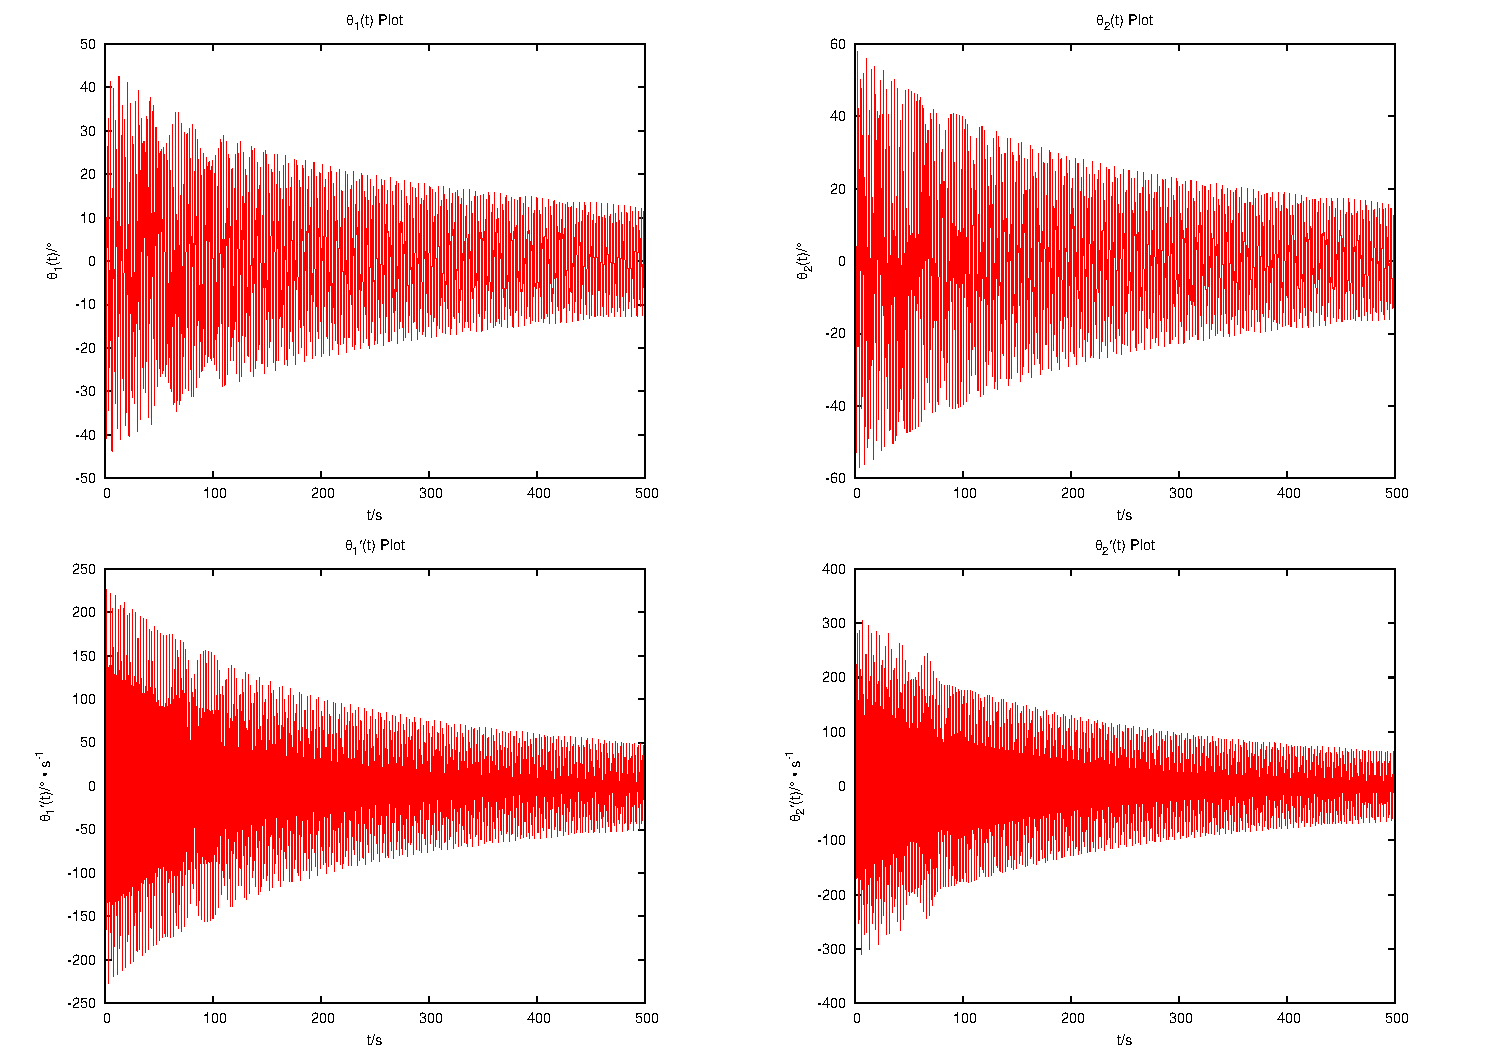
\includegraphics[width=0.8\textwidth]{./rss1move.pdf}
\caption[Caption for LOF]{空气阻尼系数$\mu=0.01$时的运动-时间曲线}
\label{fig:rss1move}
\end{figure}
\begin{figure}[H]
\centering
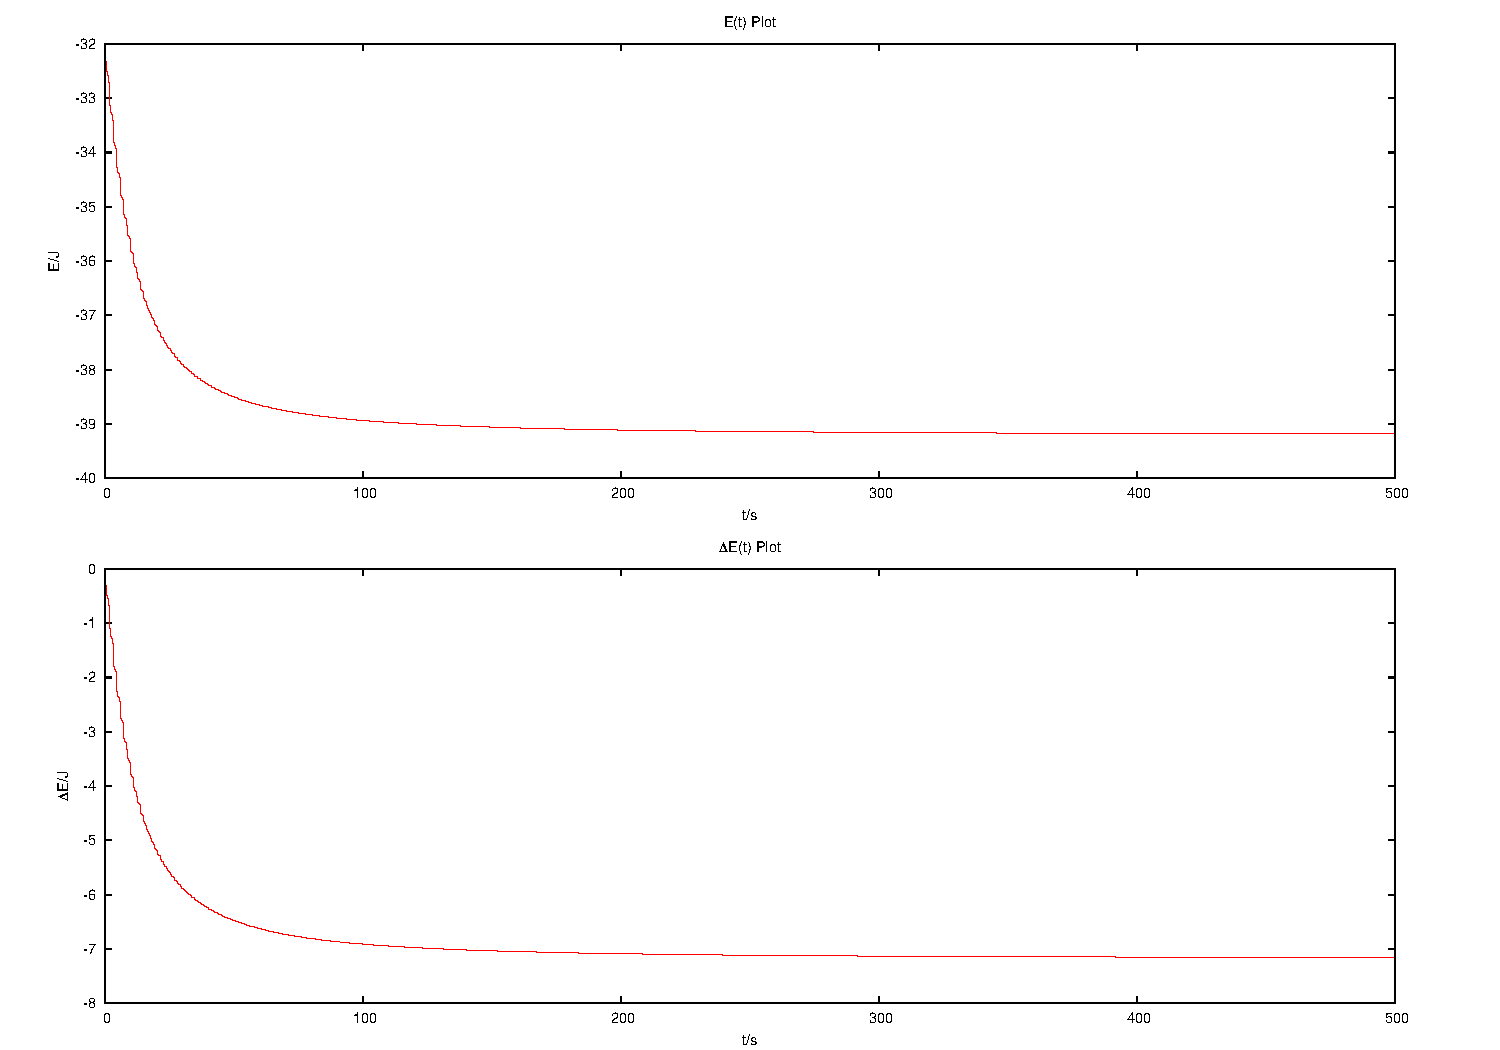
\includegraphics[width=0.8\textwidth]{./rss2E.pdf}
\caption[Caption for LOF]{空气阻尼系数$\mu=0.1$时的能量-时间曲线}
\label{fig:rss2E}
\end{figure}
\begin{figure}[H]
\centering
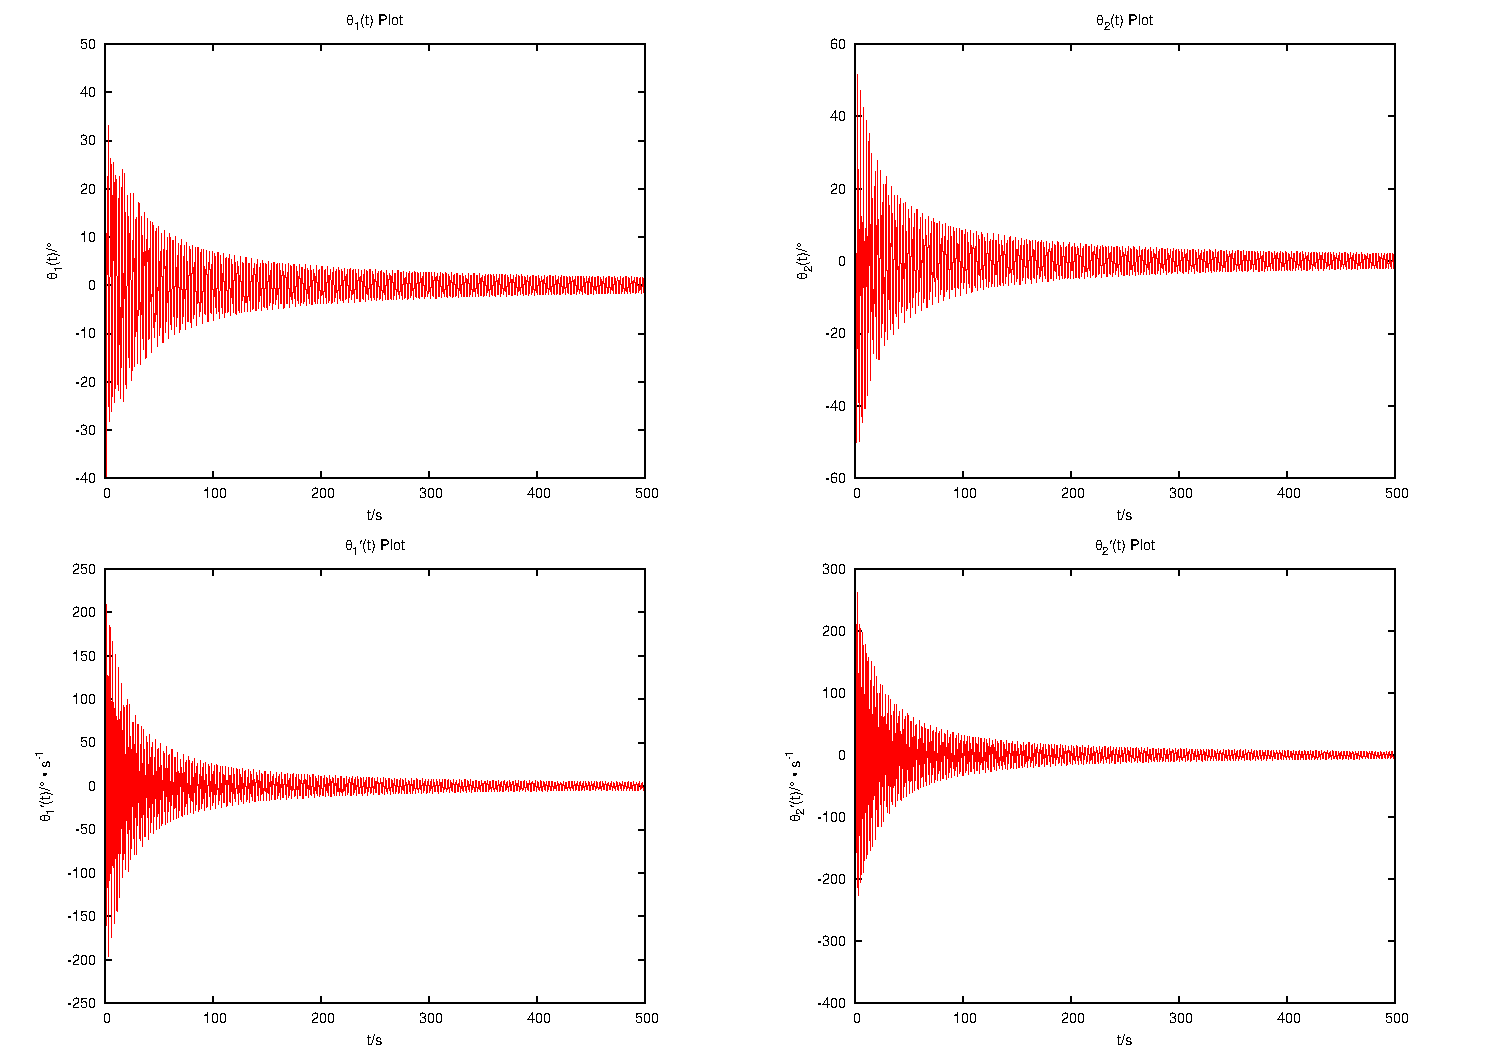
\includegraphics[width=0.8\textwidth]{./rss2move.pdf}
\caption[Caption for LOF]{空气阻尼系数$\mu=0.1$时的运动-时间曲线}
\label{fig:rss2move}
\end{figure}

从不同的$\mu$值的模拟结果可以看出,由于空气阻力会导致系统能量不断耗散,因此系统的能量曲线为下降趋势,同样,运动曲线的包络线也为收缩趋势。并且空气阻尼系数$\mu$越大,能量下降趋势和运动包络线的收缩趋势越明显,与理论预期相同。

由于空气阻力与速度大小的关系
\begin{equation}
	\vec{f}=-\mu \frac{(\vec{v}\cdot\hat{\theta})^3}{|\vec{v}\cdot\hat{\theta}|} \notag
\end{equation}
为二次曲线关系,因此当摆的运动速度较低时,空气阻力的影响不明显。这一点在图~\ref{fig:rss2move}中反应较明显,即当摆角较小,角速度较低时,由于空气阻力影响很小,摆的运动与无空气阻力情况接近。

\section{结论}
经过利用Verlet算法、经典Runge-Kutta算法、自适应时间步长算法对于双杆复合摆系统的计算,分别计算了无空气阻力系统和有空气阻力系统,对于数值模拟算法和两种情况双杆摆系统得出如下结论
\begin{enumerate}
	\item Verlet算法仅适用于简单的、条件不极端的短时模拟系统。对于模拟时间较长、初始条件极端的系统,采用经典Runge-Kutta算法的计算精度更高,收敛性更好,且可以很大程度上减少累积误差;
	\item 自适应时间步长算法是一种对于经典Runge-Kutta算法的改进算法。该算法具有自动平衡计算精度和计算时间的能力,同时对于条件变化较为极端、长时模拟及对于经典Runge-Kutta算法收敛性较差的系统有较好的全局精度;
	\item 若考虑满足二次形式的空气阻尼,双杆摆系统的能量随时间不断降低,并趋于极小值(即系统的静态最低能量点),能量和运动包络线随时间的下降速度不断降低,最终趋于0。
\end{enumerate}

\clearpage
\addcontentsline{toc}{section}{参考文献}
\begin{thebibliography}{99}
	\bibitem{Huang} 黄维诚. 分析力学讲义[M]. 北京: 清华大学理学院, 2011: 62-78
	\bibitem{Guan} 关治, 陆金甫. 数值分析基础(第二版)[M]. 北京: 高等教育出版社, 2010: 358-368, 397-401 
	\bibitem{Garcia} Alejandro L. Garcia. Numerical Methods for Physics[M]. Englewood Cliffs, New Jersey: Prentice Hall, 1994: 72-73 
	\bibitem{William} William H. Press, Brian P. Flannery, Saul A. Teukolsky, William T. Vetterling. Numerical Recipes: the Art of Scientific Computing[M]. Cambridge: Cambridge University Press, 1986: 554-558 
\end{thebibliography}


\end{document}